\chapter{Desarrollo}
\label{develop}

El desarrollo del emulador se estructura en diversas fases que abordan los \textbf{principales componentes de la consola}, comenzando por la CPU, continuando con la gestión de gráficos (GPU/PPU) y memoria (RAM/ROM), y concluyendo con la implementación de las interfaces de entrada y salida (I/O). Cada uno de estos módulos es fundamental para asegurar una emulación fiel al hardware original, por lo que se prestará \textbf{especial atención a la precisión y al rendimiento}.
\\\\
La \textbf{primera fase} se centrará en la \textbf{implementación de la CPU}, que es responsable de ejecutar las instrucciones del juego. Cada paso del desarrollo irá acompañado de \textbf{pruebas y validaciones} para garantizar que el emulador reproduzca el comportamiento de la consola original de manera eficiente. Esto último se conseguirá mediante la implementación de \textbf{pruebas unitarias} que verifiquen el correcto comportamiento de los opcodes.

\section{Módulos / Estructura del Proyecto}

El emulador que se va a implementar constará de \textbf{distintos módulos}, cada uno con una \textbf{función específica} y clara, lo que facilitará tanto su comprensión como el desarrollo de cada uno de los aspectos del emulador. A continuación, se describen brevemente los \textbf{módulos principales del proyecto}:

\begin{itemize} 
    \item \textbf{Emulator}: Este módulo centraliza la gestión de los otros componentes, coordinando su interacción y asegurando que el ciclo de emulación se ejecute correctamente. Controla el flujo general del programa.
    \item \textbf{CPU}: Responsable de la ejecución de las instrucciones. Se encarga de la implementación del conjunto de instrucciones de la Game Boy y la simulación de los registros, el Program Counter (PC), el Stack Pointer (SP) y las operaciones con la ALU.
    \item \textbf{Memory}: Gestiona el acceso a la memoria principal del sistema. Proporciona una interfaz para leer y escribir datos en las distintas áreas de la memoria del emulador, incluyendo ROM, RAM y áreas de E/S.
    \item \textbf{ROM}: Módulo encargado de cargar y gestionar la memoria ROM, que contiene el código del juego o programa a emular. Lee los datos directamente desde el archivo del juego y los pone a disposición del emulador.
    \item \textbf{RAM}: Controla la memoria de acceso aleatorio del sistema, donde se almacenan temporalmente datos durante la ejecución del programa. Es volátil y se borra cada vez que se reinicia el sistema.
    \item \textbf{PPU (Pixel Processing Unit)}: Se encarga de la representación gráfica. Simula la unidad de procesamiento de píxeles de la consola, manejando la creación y renderización de sprites y fondos en pantalla.
    \item \textbf{Timer}: Simula los temporizadores de la consola, necesarios para sincronizar eventos y gestionar interrupciones relacionadas con el tiempo, como el reloj del sistema y los temporizadores de la CPU.
    \item \textbf{Interrupt}: Maneja las interrupciones generadas por los eventos del sistema, como teclas presionadas, cambios en el PPU o eventos de temporización. Se encarga de priorizarlas y derivarlas a las funciones correspondientes.
    \item \textbf{IO (Input/Output)}: Administra las interacciones de entrada y salida, como las pulsaciones de los botones del usuario y la comunicación con dispositivos externos.
    \item \textbf{DMA}: Permite la transferencia de datos entre la memoria de vídeo y la memoria principal sin la intervención del CPU. Facilita la copia eficiente de gráficos y sprites, optimizando el rendimiento al liberar al CPU para otras tareas durante las transferencias de datos.
    \item \textbf{FifoFetcher}: Gestiona la recuperación de datos de píxeles de la memoria de video, utilizando una estructura FIFO para almacenar temporalmente la información de tiles y atributos. Su función principal es asegurar una carga eficiente de píxeles para la representación gráfica en pantalla.
    \item \textbf{Audio}: Genera y manipula sonidos en la Game Boy, gestionando canales de audio como ondas de pulso y ruido. Controla la frecuencia, duración y mezcla de los sonidos.
\end{itemize}

\section{CPU}

El desarrollo comienza con la implementación de la \textbf{Unidad Central de Procesamiento}. Debido a su papel fundamental en la correcta reproducción del funcionamiento del sistema, esta etapa se centra en \textbf{implementar todas las instrucciones} para asegurar que el emulador pueda procesar cada byte de información con precisión.

\subsection{Registros}
Para definirlos en nuestro programa, \textbf{utilizaremos el tipo Byte} o UByte de Kotlin. En mi caso por desconocimiento del segundo tipo, comencé a programarlo con Byte. La diferencia entre ambos es que Byte utiliza el rango de [-128:128] y UByte el de [0:255] (igual que la GB). Podemos hacer uso de cualquiera de los dos mientras tengamos en mente que, si el primero lo convertimos a Integer, será un valor distinto al original. \textbf{En cuanto a PC y SP}, optaremos por \textbf{utilizar Integers}, ya que son \textbf{valores de 2 bytes y siempre contienen una dirección de memoria}.

\begin{lstlisting}[language=Kotlin, caption={Declaración de Registros}, label={code:kotlinregistros}]
    var A: Byte = 0
    var F: Byte = 0             // Contains the 4 flags (11110000 -> ZNHC0000)
    var B: Byte = 0
    var C: Byte = 0
    var D: Byte = 0
    var E: Byte = 0
    var H: Byte = 0
    var L: Byte = 0

    // 16 bits registers
    var SP: Int = 0xFFFE        // Stack Pointer
    var PC: Int = 0             // Program Counter
\end{lstlisting}

\textbf{Para operar con ellos a nivel de byte}, deberemos \textbf{pasarlos a Integer}, aplicarles una \textbf{operación AND con el valor 0xFF} (para eliminar el signo en caso de se utilice el tipo Byte originalmente), se ejecutarían las operaciones necesarias y al \textbf{resultado se le aplicaría el mismo AND}, para justo después \textbf{volver a convertirlo a Byte}:

\begin{lstlisting}[language=Kotlin, caption={Ejemplo de Opcode}, label={code:kotlinexample}]
    fun add_a_c(): Int{
        val intA = A.toInt() and 0xFF // Conversión de Byte a Integer sin signo -> A
        val intC = C.toInt() and 0xFF // Conversión de Byte a Integer sin signo -> C
        val result = intA + intC // Se suman ambos valores (ADD)
        A = (result and 0xFF).toByte() // Al resultado se le quita el signo por precaución y se convierte a Byte

        updateAddOperationFlags(intA, intC, result) // Se actualizan los Flags correspondientes

        return CYCLES_4 // Devolvemos los ciclos que la CPU debe tardar en ejecutar la instrucción
    }
\end{lstlisting}

Para la \textbf{actualización de los flags}, se implementarán \textbf{funciones específicas que gestionarán su estado} de manera adecuada. Adicionalmente, se declararán constantes que facilitarán la identificación del estado de cada flag en cualquier momento. Estas constantes corresponden a los bits asociados con un valor de 1 en formato hexadecimal (por ejemplo, 0x80 corresponde a 0b10000000).

\begin{lstlisting}[language=Kotlin, caption={Actualización de Flags}, label={code:kotlinflags}]

    // Flags --> Booleans
    const val FLAG_Z = 0x80           // Zero Flag
    const val FLAG_N = 0x40           // Subtract Flag
    const val FLAG_H = 0x20           // Half Carry Flag
    const val FLAG_C = 0x10           // Carry Flag

    [...]

    fun setFlag(flag: Int) {
        F = (F.toInt() or flag).toByte()
    }

    fun clearFlag(flag: Int) {
        F = (F.toInt() and flag.inv()).toByte()
    }

    fun updateFlag(flag: Int, condition: Boolean) {
        if (condition) {
            setFlag(flag)
        } else {
            clearFlag(flag)
        }
    }

    fun flagIsSet(flag: Int): Boolean{
        return (F.toInt() and flag) != 0
    }
\end{lstlisting}

\subsection{Opcodes}

Lo primero es \textbf{identificar qué operación ejecutar dependiendo del byte} que nos llegue. Podemos hacerlo de muchas maneras, en este caso lo vamos a manejar mediante un switch:

\begin{lstlisting}[language=Kotlin, caption={Identificación de Opcode}, label={code:kotlinwhen}]
    fun execute(opcode: Byte): Int {
        return when (opcode.toInt() and 0xFF) {
            0x00 -> nop()
            0x01 -> ld_bc_nn()              // LD BC, nn
            0x02 -> ld_bc_a()               // LD [BC], A
            0x03 -> inc_bc()                // INC BC
            0x04 -> inc_b()                 // INC B
            0x05 -> dec_b()                 // DEC B
            0x06 -> ld_b_n()                // LD B, n

            [...]

            0xFA -> ld_a_nn()               // LD A, [NN]
            0xFB -> ei()                    // EI
            0xFE -> cp_n()                  // CP N
            0xFF -> rst(0x0038)             // RST 38H
            else -> throw IllegalArgumentException("Instruction not supported: ${opcode.toInt() and 0xFF}")
        }
    }       
\end{lstlisting}

Para las \textbf{instrucciones extendidas}, se implementará otro switch que, de la misma forma, hará también distinción por Byte, pero al que solamente se llegará en caso de que en este primero encontremos el \textbf{Byte 0xCB}.
\\\\
En caso de que el input que nos llegue por parámetro no represente ninguna instrucción conocida, el emulador lanzará una excepción y finalizará la ejecución.
\\\\
Por cada instrucción, como ya hemos visto, deberemos tener en cuenta las características mencionadas previamente. Vamos a mostrar \textbf{ejemplos de instrucciones} ya implementadas por cada categoría:

\paragraph{Funciones comunes:}
Algunas funciones comunes que la gran mayoría de instrucciones van a utilizar.

\begin{lstlisting}[language=Kotlin, caption={Operaciones comunes}, label={code:kotlincommon}]
    fun fetch(): Byte {
        val byte = Memory.getByteOnAddress(PC)

        if(!cpu_halt_bug){
            PC = (PC + 1) and 0xFFFF
        }else{
            cpu_halt_bug = false
        }

        return byte
    }

    fun fetch16(): Int {
        val low = fetch().toInt() and 0xFF
        val high = fetch().toInt() and 0xFF
        return return get_16bit_address(high, low)
    }

    fun get_16bit_address(high: Byte, low: Byte): Int{
        return ((high.toInt() and 0xFF) shl 8) or (low.toInt() and 0xFF)
    }

    fun set_16bit_address_value(high: Byte, low: Byte, value: Byte){
        val address = get_16bit_address(high, low)
        Memory.writeByteOnAddress(address, value)
    }
\end{lstlisting}

La \textbf{función \textit{fetch()}} tiene como objetivo principal \textbf{obtener el byte almacenado en la dirección de memoria señalada por el PC}, e incrementarlo posteriormente (si no se produce el fallo de la CPU, que será explicado más adelante). 
\\\\
Por su parte, \textbf{\textit{fetch16()} realiza dos llamadas consecutivas a \textit{fetch()}} y combina los dos bytes obtenidos mediante la función \textit{get\_16bit\_address()}, que utiliza las operaciones SHL y OR. 
\\\\
Finalmente, la función \textit{set\_16bit\_address\_value()}, recibe una dirección como parámetro y delega al módulo de memoria la escritura del valor proporcionado, si es posible hacerlo.

\paragraph{Carga - LD:}\label{instrLd}

Añadimos de ejemplo cuatro funciones de las cuales podemos derivar el resto. En todos ellos se van a devolver los ciclos de reloj correspondientes.

\begin{lstlisting}[language=Kotlin, caption={Operaciones LD}, label={code:kotlinld}]
    fun ld_c_l(): Int{
        C = L
        return CYCLES_4
    }

    fun ld_c_hl(): Int{
        val hl = get_16bit_address(H, L)
        C = Memory.getByteOnAddress(hl)
        return CYCLES_8
    }

    fun ld_hl_b(): Int{
        set_16bit_address_value(H, L, B)
        return CYCLES_8
    }

    fun ld_hl_nn(): Int{
        val low = fetch().toInt() and 0xFF
        val high = fetch().toInt() and 0xFF
        H = high.toByte()
        L = low.toByte()

        return CYCLES_12
    }
\end{lstlisting}

En la primera función (LD C, L) simplemente se carga el contenido del registro L en C.
\\\\
En la siguiente (LD C, [HL]) lo que se debe hacer es obtener el byte almacenado en la dirección de memoria señalada por HL y cargarlo en C (para ello hacemos uso del módulo de memoria).
\\\\
La tercera función (LD [HL], B) es justo lo contrario a la segunda. En este caso lo que hacemos es guardar el byte del registro B en la dirección de memoria ya especificada en HL.
\\\\
Por último, en la cuarta función (LD [HL], NN), no nos viene especificado un registro, si no que debemos obtener los dos siguientes bytes del PC. Hay que recordar que los bytes se guardan en memoria en \textbf{Little Endian}, por lo que el primero que se obtiene es el Low. Asignamos al registro H el High y al registro L el Low, y al devolver los ciclos correspondientes quedaría implementada la instrucción.

\paragraph{Aritméticas y Lógicas:} En esta categoría entran todas las \textbf{instrucciones de ADD, ADC, AND, SUB, SBC, DEC, INC, XOR, OR, CP, CPL, CCF, DAA y SCF}. Vamos a ver algunos ejemplos de cada una de ellas:

\begin{lstlisting}[language=Kotlin, caption={Operaciones ADD y ADC}, label={code:kotlinaddc}]
    fun updateAddOperationFlags(val1: Int, val2: Int, result: Int){
        updateFlag(FLAG_Z, result == 0)
        clearFlag(FLAG_N)
        updateFlag(FLAG_H, (val1 and 0xF) + (val2 and 0xF) > 0xF)
        updateFlag(FLAG_C, result > 0xFF)
    }

    fun add_a_b(): Int{
        val intA = A.toInt() and 0xFF
        val intB = B.toInt() and 0xFF
        val result = intA + intB
        A = (result and 0xFF).toByte()

        updateAddOperationFlags(intA, intB, result)

        return CYCLES_4
    }

    fun adc_a_b(): Int{
        val carry = if (flagIsSet(FLAG_C)) 1 else 0
        val intA = A.toInt() and 0xFF
        val intB = B.toInt() and 0xFF
        val result = intA + (intB + carry)
        A = (result and 0xFF).toByte()

        updateAddOperationFlags(intA, intB + carry, result)

        return CYCLES_4
    }
\end{lstlisting}

Para la instrucción \textbf{ADD} (en este caso \textbf{ADD A, B}), la operación consiste en convertir ambos registros a enteros sin signo y sumar sus valores.
\\\\
La \textbf{diferencia entre ADD y ADC} reside en que en \textbf{este último al resultado también se le suma el valor del carry} y, por ende, se debe tener en cuenta en la actualización del flag Half-Carry.
\\\\
En los casos que impliquen el uso de direcciones de memoria (operaciones de 2 bytes), se puede emplear el código utilizado en las instrucciones de carga (LD) \ref{instrLd} como referencia.

\begin{lstlisting}[language=Kotlin, caption={Operaciones INC y DEC}, label={code:kotlinincdec}]
    fun inc_8bit_register(register: Byte): Byte{
        val toReturn = (register.toInt() + 1).toByte()
        updateFlag(FLAG_Z, toReturn.toInt() == 0x00)
        clearFlag(FLAG_N)
        updateFlag(FLAG_H, ((register.toInt() and 0xF) + 1) and 0x10 != 0x00)
        return toReturn
    }

    fun dec_8bit_register(register: Byte): Byte{
        val toReturn = (register.toInt() - 1).toByte()
        updateFlag(FLAG_Z, toReturn.toInt() == 0x00)
        setFlag(FLAG_N)
        updateFlag(FLAG_H, (register.toInt() and 0xF == 0x00))
        return toReturn
    }

    fun inc_bc(): Int{
        val oldValue = get_16bit_address(B, C)
        val newValue = (oldValue + 1) and 0xFFFF
        B = (newValue shr 8).toByte()
        C = newValue.toByte()
        return CYCLES_8
    }

    fun dec_b(): Int{
        B = dec_8bit_register(B)
        return CYCLES_4
    }

    fun inc_b(): Int{
        B = inc_8bit_register(B)
        return CYCLES_4
    }
\end{lstlisting}

Las instrucciones de INC y DEC son muy similares. \textbf{INC suma 1 al valor} y afecta los flags del procesador: el Zero (Z) se activa si el resultado es 0, el Half-carry (H) se activa si hay un acarreo entre los bits 3 y 4, y el Subtract (N) siempre se borra. Por su parte, \textbf{DEC resta 1 al valor} y afecta los mismos flags, pero siempre activa el Subtract (N) ya que es una operación de sustracción. Ambos opcodes no afectan el Carry flag (C) y se utilizan tanto para registros de 8 bits como para posiciones de memoria.

\begin{lstlisting}[language=Kotlin, caption={Operación XOR}, label={code:kotlinxor}]
    fun xor_b(): Int{
        A = (((A.toInt() and 0xFF) xor (register.toInt()) and 0xFF)).toByte()

        updateFlag(FLAG_Z, (A.toInt() and 0xFF) == 0)
        clearFlag(FLAG_N)
        clearFlag(FLAG_H)
        clearFlag(FLAG_C)
        
        return CYCLES_4
    }
\end{lstlisting}

La \textbf{operación XOR} se realizan \textbf{siempre al registro A}, utilizando su valor y el del registro indicado por el opcode (en este caso B). Tras la operación, verifica si el resultado es cero para activar el flag Z, y limpia los flags N, H y C, ya que no son relevantes.
\\\\
Las operaciones OR son idénticas en Kotlin, simplemente deberemos cambiar el operando 'xor' por 'or'.

\paragraph{Control de flujo:} Las \textbf{instrucciones de control de flujo}, como CALL, JP y RETI, \textbf{permiten modificar la secuencia de ejecución del programa}. Estas instrucciones desvían el flujo normal de instrucciones al saltar a direcciones específicas de memoria o retornar desde subrutinas o interrupciones. Tenemos instrucciones como CALL, JP o JR que son utilizadas para saltar a una nueva dirección, con CALL almacenando la dirección de retorno en la pila para permitir volver al punto de origen.
\\\\
Vamos a analizarlas de una en una:
\begin{lstlisting}[language=Kotlin, caption={Operación CALL}, label={code:kotlincall}]
    fun call_nz_nn(): Int{
        val address = fetch16()

        if (!flagIsSet(FLAG_Z)) {
            SP = (SP - 1) and 0xFFFF
            Memory.writeByteOnAddress(SP, (PC ushr 8).toByte()) // Alto
            SP = (SP - 1) and 0xFFFF
            Memory.writeByteOnAddress(SP, (PC and 0xFF).toByte()) // Bajo
    
            PC = address
            return CYCLES_24
        }

        return CYCLES_12
    }
\end{lstlisting}

La instrucción \textbf{CALL salta a una subrutina especificada}, guardando la dirección de retorno en la pila. El PC se actualiza con la dirección de destino, y tras ejecutar la subrutina, el programa puede volver al punto original usando la instrucción RET, restaurando la dirección desde la pila. Esta último instrucción no se implementa en el propio CALL, si no que debe ser gestionada a posterior por parte del desarrollador, utilizando el valor previo del PC (guardado en el SP antes de su actualización).
\\\\
Además, en el ejemplo expuesto, se nos indica que el CALL solamente se debe ejecutar si el Flag Z no está activo. En caso contrario, lo único que haría son 2 \textit{fetch()} seguidos y se hace uso de menos ciclos de reloj.

\begin{lstlisting}[language=Kotlin, caption={Operaciones JR y JP}, label={code:kotlinjpjr}]
    fun jr_n(): Int{
        val offset = fetch()
        PC += offset.toInt()
        return CYCLES_12
    }

    fun jp_nn(): Int{
        val address = fetch16()
        PC = address
        return CYCLES_16
    }
\end{lstlisting}

Las instrucciones \textbf{JR} y \textbf{JP} son similares a CALL, pero no almacenan el valor actual del PC en el stack. 
\\\\
La instrucción \textbf{JP salta directamente a una dirección de memoria especificada}, actualizando el PC, lo que permite saltos largos a cualquier posición en la memoria. 
\\\\
\textbf{JR}, en cambio, realiza un \textbf{salto relativo}, ajustando el PC en función de un desplazamiento positivo o negativo, permitiendo saltos más cortos dentro de un rango cercano. Dado que los saltos relativos pueden cubrir un \textbf{máximo de 0xFF bytes} hacia arriba o abajo, \textbf{JR consume menos ciclos de reloj}.

\begin{lstlisting}[language=Kotlin, caption={Operaciones RET y RETI}, label={code:kotlinreti}]
    fun executeRetOperation(){
        val low = Memory.getByteOnAddress(SP).toInt() and 0xFF
        SP = (SP + 1) and 0xFFFF
        val high = Memory.getByteOnAddress(SP).toInt() and 0xFF
        SP = (SP + 1) and 0xFFFF

        PC = (high shl 8) or low
    }

    fun ret(): Int{
        executeRetOperation()
        return CYCLES_16
    }

    fun reti(): Int{
        executeRetOperation()
        Interrupt.enableInterrupts(true)
        return CYCLES_16
    }
\end{lstlisting}

Las instrucciones \textbf{RET} y \textbf{RETI} se utilizan para \textbf{retornar de una subrutina}, recuperando la dirección de retorno almacenada en el stack. RET restaura el valor del registro PC desde el stack, permitiendo así continuar la ejecución desde donde se dejó al llamar a la subrutina. En contraste, \textbf{RETI} realiza la misma operación, pero se utiliza específicamente para el \textbf{retorno de una interrupción}, asegurando que se manejen correctamente las interrupciones pendientes antes de restaurar el flujo de ejecución.

\begin{lstlisting}[language=Kotlin, caption={Operación CP}, label={code:kotlincp}]
    fun cp_b(): Int{
        val intA = A.toInt() and 0xFF
        val intRegister = B.toInt() and 0xFF

        val result = (intA - intRegister) and 0xFF

        updateFlag(FLAG_Z, result == 0)
        setFlag(FLAG_N)
        updateFlag(FLAG_H, (intA and 0xF) < (intRegister and 0xF))
        updateFlag(FLAG_C, intA < intRegister)
        
        return CYCLES_4
    }
\end{lstlisting}

La función \textbf{CP B} (Compare B) se encarga de \textbf{comparar el valor del registro A con el valor del registro B}, estableciendo los flags correspondientes según el resultado de la comparación. Primero, convierte los registros A y B a enteros de 8 bits, luego calcula el resultado de la resta entre A y B, enmascarando el resultado para asegurarse de que se mantenga dentro del rango de 8 bits. A continuación, actualiza el flag Z si el resultado es igual a cero, establece el flag N para indicar que se realizó una comparación, y determina el estado del flag H al verificar si el nibble menos significativo de A es menor que el de B. Por último, establece el flag C si el valor de A es menor que el de B.

\begin{lstlisting}[language=Kotlin, caption={Operación CPL}, label={code:kotlincpl}]
    fun cpl(): Int{

        A = (A.toInt() xor 0xFF).toByte()

        setFlag(FLAG_N)
        setFlag(FLAG_H)

        return CYCLES_4
    }
\end{lstlisting}

La \textbf{función CPL} (Complementary) se encarga de \textbf{complementar el valor del registro A, invirtiendo todos sus bits mediante una operación XOR con 0xFF}. Esto transforma todos los bits de A en sus opuestos, cambiando ceros por unos y viceversa. Después de realizar la operación, la función establece el flag N para indicar que se ha realizado una operación que afecta al signo del número, y también establece el flag H para indicar que puede haber un acarreo en la operación.

\begin{lstlisting}[language=Kotlin, caption={Operación CCF}, label={code:kotlinccf}]
    fun ccf(): Int{

        val newCarry = ((F.toInt() and 0xFF) and FLAG_C) == 0
        updateFlag(FLAG_C, newCarry)
        setFlag(FLAG_N)
        setFlag(FLAG_H)

        return CYCLES_4
    }
\end{lstlisting}

La \textbf{función CCF} (Complement Carry Flag) se encarga de \textbf{complementar el valor del flag C}. Primero, verifica si el flag de acarreo está actualmente activado; si no lo está, lo activa, y si lo está, lo desactiva, utilizando el operador lógico AND para determinar su estado anterior. Además, establece los flags H y N como activos.

\begin{lstlisting}[language=Kotlin, caption={Operación DAA}, label={code:kotlindaa}]
    fun daa(): Int{

        var result = A.toInt() and 0xFF

        if (!flagIsSet(FLAG_N)) { // Addition

            if ((result and 0x0F) > 9 || flagIsSet(FLAG_H)) // Lower nibble
                result += 0x06

            if ((result and 0xF0) > 0x90 || flagIsSet(FLAG_C)) // Higher nibble
                result += 0x60

        }else{ // Substraction
            if (flagIsSet(FLAG_H)) // Lower nibble
                result -= 0x06

            if (flagIsSet(FLAG_C)) // Higher nibble
                result -= 0x60
        }

        updateFlag(FLAG_Z, (result and 0xFF) == 0x00)
        clearFlag(FLAG_H)
        updateFlag(FLAG_C, result > 0xFF)

        result = result and 0xFF
        A = result.toByte()

        return CYCLES_4
    }
\end{lstlisting}

La \textbf{función DAA} (Decimal Adjust for Addition) es una implementación que \textbf{ajusta el valor del registro A para operaciones aritméticas en formato decimal} después de una suma o resta. El método primero convierte el valor de A a un entero de 8 bits, luego verifica si la operación anterior fue una suma o una resta basándose en el estado del flag N.

\begin{lstlisting}[language=Kotlin, caption={Operación SCF}, label={code:kotlinscf}]
    fun scf(): Int{

        clearFlag(FLAG_N)
        clearFlag(FLAG_H)
        setFlag(FLAG_C)

        return CYCLES_4
    }
\end{lstlisting}

La \textbf{función SCF} (Set Carry Flag) \textbf{establece el flag C a 1 y borra los flags N y H}, lo que indica que el próximo cálculo tendrá en cuenta que se ha producido un acarreo.

\paragraph{Rotación y desplazamiento:} En esta categoría tenemos las \textbf{instrucciones de RL, RR, RLC, RRC, SLA, SRA, SWAP y SRL}. Vamos a ver algunos ejemplos de cada una de ellas:

\begin{lstlisting}[language=Kotlin, caption={Operaciones RL y RR}, label={code:kotlinrlrr}]
    fun rl_b(): Int{
        val bByte = B.toInt() and 0xFF
        val oldCarry = if (flagIsSet(FLAG_C)) 1 else 0
        val newCarry = (bByte ushr 7) and 0x1

        B = ((bByte shl 1) or oldCarry).toByte()

        updateFlag(FLAG_Z, B == 0.toByte())
        clearFlag(FLAG_N)
        clearFlag(FLAG_H)
        updateFlag(FLAG_C, newCarry == 1)

        return CYCLES_8
    }
    
    fun rr_b(): Int{
        val bByte = B.toInt() and 0xFF
        val oldCarry = if (flagIsSet(FLAG_C)) 1 else 0
        val newCarry = (bByte ushr 7) and 0x1

        B = ((bByte shr 1) or (oldCarry shl 7)).toByte()

        updateFlag(FLAG_Z, B == 0.toByte())
        clearFlag(FLAG_N)
        clearFlag(FLAG_H)
        updateFlag(FLAG_C, newCarry == 1)

        return CYCLES_8
    }
\end{lstlisting}

Las \textbf{funciones RL B y RR B realizan rotaciones de bits en el registro B}, pero difieren en la dirección y el manejo del carry. La \textbf{función RL rota los bits hacia la izquierda}; el MSB se desplaza a la izquierda y se introduce en el LSB, utilizando el valor del carry anterior para completar la rotación. En cambio, \textbf{RR rota los bits hacia la derecha}; el LSB se mueve al carry y el carry anterior se coloca en el MSB. Ambas funciones actualizan los indicadores de estado, como el flag Z si el resultado es cero, y el flag C según el bit que se desplaza.

\begin{lstlisting}[language=Kotlin, caption={Operaciones RLC y RRC}, label={code:kotlinrlcrrc}]
    fun rlc_b(): Int{
        val bByte = B.toInt() and 0xFF
        val carry = (bByte ushr 7) and 0x1
        B = ((bByte shl 1) or carry).toByte()

        updateFlag(FLAG_Z, B == 0.toByte())
        clearFlag(FLAG_N)
        clearFlag(FLAG_H)
        updateFlag(FLAG_C, carry == 1)

        return CYCLES_8
    }

    fun rrc_b(): Int{
        val bByte = B.toInt() and 0xFF
        val carry = bByte and 0x1
        B = ((bByte shr 1) or (carry shl 7)).toByte()

        updateFlag(FLAG_Z, B == 0.toByte())
        clearFlag(FLAG_N)
        clearFlag(FLAG_H)
        updateFlag(FLAG_C, carry == 1)

        return CYCLES_8
    }
\end{lstlisting}

La \textbf{función RLC B} realiza una \textbf{rotación a la izquierda del registro B}, desplazando el MSB hacia el LSB y estableciendo el nuevo valor del MSB en el carry. Actualiza todos los flags en función del resultado. En contraste, la función RRC B efectúa una rotación a la derecha, desplazando el LSB hacia el MSB y estableciendo su nuevo valor en el carry.

\begin{lstlisting}[language=Kotlin, caption={Operaciones SLA, SRA y SRL}, label={code:kotlinslasrasrl}]
    fun sla_b(): Int{
        val bByte = B.toInt() and 0xFF
        val newCarry = (bByte ushr 7) and 0x1
        B = ((bByte shl 1) and 0xFE).toByte()

        updateFlag(FLAG_Z, B == 0.toByte())
        clearFlag(FLAG_N)
        clearFlag(FLAG_H)
        updateFlag(FLAG_C, newCarry == 1)
        
        return CYCLES_8
    }

    fun sra_b(): Int{
        val bByte = B.toInt() and 0xFF
        val oldBit7 = bByte and 0x80
        val newCarry = bByte and 0x1

        B = ((bByte shr 1) or oldBit7).toByte()

        updateFlag(FLAG_Z, B == 0.toByte())
        clearFlag(FLAG_N)
        clearFlag(FLAG_H)
        updateFlag(FLAG_C, newCarry == 1)

        return CYCLES_8
    }

    fun srl_b(): Int{
        val bByte = B.toInt() and 0xFF
        val newCarry = bByte and 0x1
        B = ((bByte shr 1) and 0x7F).toByte()

        updateFlag(FLAG_Z, B == 0.toByte())
        clearFlag(FLAG_N)
        clearFlag(FLAG_H)
        updateFlag(FLAG_C, newCarry == 1)

        return CYCLES_8
    }
\end{lstlisting}

La \textbf{función SLA B} realiza un \textbf{desplazamiento lógico a la izquierda del registro B}, moviendo todos los bits una posición a la izquierda y estableciendo el LSB en 0, mientras que el nuevo carry se toma del antiguo MSB. En contraste, \textbf{SRA B realiza un desplazamiento aritmético a la derecha}, manteniendo el bit más significativo y moviendo el resto de los bits hacia la derecha, con el nuevo carry tomado del antiguo LSB. Por otro lado, \textbf{SRL B} también \textbf{realiza un desplazamiento lógico a la derecha}, pero establece el MSB en 0 y mueve los bits a la derecha, con el nuevo carry tomado del antiguo LSB.

\begin{lstlisting}[language=Kotlin, caption={Operación SWAP}, label={code:kotlinswap}]
    fun swap_b(): Int{
        val bByte = B.toInt() and 0xFF
        val low = (bByte and 0x0F) shl 4
        val high = (bByte and 0xF0) shr 4
        B = (low or high).toByte()

        updateFlag(FLAG_Z, B == 0.toByte())
        clearFlag(FLAG_N)
        clearFlag(FLAG_H)
        clearFlag(FLAG_C)

        return CYCLES_8
    }
\end{lstlisting}

La \textbf{función SWAP B intercambia los nibbles (4 bits) del registro B}, moviendo los 4 bits menos significativos a la posición de los 4 bits más significativos y viceversa. Actualiza el flag Z si el nuevo valor es cero, y limpia los flags N, H y C.

\paragraph{Manipulación de bits:} Encontramos las instrucciones BIT, RES y SET.

\begin{lstlisting}[language=Kotlin, caption={Operación BIT}, label={code:kotlinbit}]
    fun updateBitOperationFlags(result: Boolean){
        updateFlag(FLAG_Z, result)
        clearFlag(FLAG_N)
        setFlag(FLAG_H)
    }

    fun bit_operation(register: Int, bitNumber: Int): Int{

        require(bitNumber in 0..7) { "Bit must be between 0 and 7" }
        require(register in 1..8) { "Register must be between 1 and 8" }

        var bitZero = false
        var cyclesToReturn = CYCLES_8
        val bit = 0x1 shl bitNumber

        when (register) {
            1 -> bitZero = ((B.toInt() and 0xFF) and bit) == 0
            2 -> bitZero = ((C.toInt() and 0xFF) and bit) == 0
            3 -> bitZero = ((D.toInt() and 0xFF) and bit) == 0
            4 -> bitZero = ((E.toInt() and 0xFF) and bit) == 0
            5 -> bitZero = ((H.toInt() and 0xFF) and bit) == 0
            6 -> bitZero = ((L.toInt() and 0xFF) and bit) == 0
            7 -> {
                val address = get_16bit_address(H, L)
                bitZero = ((Memory.getByteOnAddress(address).toInt() and 0xFF) and bit) == 0
                cyclesToReturn = CYCLES_16
            }
            8 -> bitZero = ((A.toInt() and 0xFF) and bit) == 0
        }

        updateBitOperationFlags(bitZero)
        return cyclesToReturn
    }
\end{lstlisting}

La \textbf{operación BIT verifica el estado de un bit específico (de 0 a 7) en un registro determinado (de 1 a 8)}. Utiliza condiciones para identificar qué registro se está evaluando y calcula si el bit indicado está apagado (0) o encendido (1). Si el registro es 7, que representa una dirección de memoria, obtiene el byte correspondiente desde esa dirección, y el tiempo de ciclo se ajusta a 16. Posteriormente, actualiza el flag Z, limpia el flag N y establece el flag H. Al final, devuelve el tiempo de ciclo correspondiente, que es 8 para los registros de 1 a 6 y el 8, y 16 para el registro 7.

\begin{lstlisting}[language=Kotlin, caption={Operación RES}, label={code:kotlinres}]
    fun res_operation(register: Int, bitNumber: Int): Int{

        require(bitNumber in 0..7) { "Bit must be between 0 and 7" }
        require(register in 1..8) { "Register must be between 1 and 8" }

        var cyclesToReturn = CYCLES_8
        val bit = (0x1 shl bitNumber).inv()

        when (register) {
            1 -> B = ((B.toInt() and 0xFF) and bit).toByte()
            2 -> C = ((C.toInt() and 0xFF) and bit).toByte()
            3 -> D = ((D.toInt() and 0xFF) and bit).toByte()
            4 -> E = ((E.toInt() and 0xFF) and bit).toByte()
            5 -> H = ((H.toInt() and 0xFF) and bit).toByte()
            6 -> L = ((L.toInt() and 0xFF) and bit).toByte()
            7 -> {
                val address = get_16bit_address(H, L)
                val result = ((Memory.getByteOnAddress(address).toInt() and 0xFF) and bit).toByte()
                Memory.writeByteOnAddress(address, result)
                cyclesToReturn = CYCLES_16
            }
            8 -> A = ((A.toInt() and 0xFF) and bit).toByte()
        }

        return cyclesToReturn
    }
\end{lstlisting}

La \textbf{operación RES} se encarga de \textbf{reiniciar (poner a 0) un bit específico (de 0 a 7) en un registro determinado} (de 1 a 8). Utiliza condiciones para determinar cuál registro se está manipulando y genera una máscara de bit que apaga el bit correspondiente. Si el registro es 7, la función obtiene la dirección de memoria desde los registros H y L, lee el byte almacenado en esa dirección, reinicia el bit correspondiente y escribe el nuevo valor de vuelta en memoria. El tiempo de ciclo se gestiona de la misma manera que en la operación BIT.

\begin{lstlisting}[language=Kotlin, caption={Operación SET}, label={code:kotlinset}]
    fun set_operation(register: Int, bitNumber: Int): Int{

        require(bitNumber in 0..7) { "Bit must be between 0 and 7" }
        require(register in 1..8) { "Register must be between 1 and 8" }

        var cyclesToReturn = CYCLES_8
        val bit = 0x1 shl bitNumber

        when (register) {
            1 -> B = ((B.toInt() and 0xFF) or bit).toByte()
            2 -> C = ((C.toInt() and 0xFF) or bit).toByte()
            3 -> D = ((D.toInt() and 0xFF) or bit).toByte()
            4 -> E = ((E.toInt() and 0xFF) or bit).toByte()
            5 -> H = ((H.toInt() and 0xFF) or bit).toByte()
            6 -> L = ((L.toInt() and 0xFF) or bit).toByte()
            7 -> {
                val address = get_16bit_address(H, L)
                val result = ((Memory.getByteOnAddress(address).toInt() and 0xFF) or bit).toByte()
                Memory.writeByteOnAddress(address, result)
                cyclesToReturn = CYCLES_16
            }
            8 -> A = ((A.toInt() and 0xFF) or bit).toByte()
        }

        return cyclesToReturn
    }
\end{lstlisting}

La \textbf{operación SET} se encarga de \textbf{establecer (poner a 1) un bit específico (de 0 a 7) en un registro determinado (de 1 a 8)}. Utiliza condiciones para identificar qué registro se está manipulando y genera una máscara de bit que activa el bit correspondiente. Si el registro es 7, la función obtiene la dirección de memoria a partir de los registros H y L, lee el byte almacenado en esa dirección, activa el bit correspondiente y escribe el nuevo valor de vuelta en la memoria. El tiempo de ciclo se gestiona de la misma manera que en la operación BIT.

\paragraph{Especiales de sistema:} Encontramos las instrucciones NOP, DI y EI:

\begin{lstlisting}[language=Kotlin, caption={Operación NOP}, label={code:kotlinnop}]
    fun nop(): Int{
        return CYCLES_4
    }
\end{lstlisting}

La \textbf{operación NOP} (No Operation) realiza una operación que \textbf{no tiene efecto en el estado del procesador}; es decir, no cambia los registros, la memoria o los flags. Su principal función es ocupar espacio en el ciclo de ejecución, permitiendo la sincronización en la ejecución de instrucciones o como un marcador para pausas en el código. A la hora de implementarlo, simplemente devolvemos los ciclos correspondientes.

\begin{lstlisting}[language=Kotlin, caption={Operaciones DI, EI}, label={code:kotlindiei}]
    private var pendingEI = false

    [...]

    fun ei(): Int{
        pendingEI = true
        return CYCLES_4
    }

    fun di(): Int{
        Interrupt.enableInterrupts(false)
        return CYCLES_4
    }
\end{lstlisting}

El \textbf{opcode EI habilita las interrupciones en el procesador} (se detallará más adelante). Es importante destacar que \textbf{las interrupciones no se activan de manera inmediata}; en su lugar, deben esperar hasta el siguiente ciclo de la CPU para entrar en efecto. Por esta razón, se utiliza una variable para almacenar el estado de las interrupciones.
\\\\
Por otro lado, \textbf{DI deshabilita las interrupciones en el procesador}, bloqueando la capacidad del sistema para responder a señales externas hasta que se vuelvan a habilitar mediante un EI. En este caso, los cambios si que tienen efecto inmediato.

\paragraph{Con pila:} Encontramos las \textbf{instrucciones PUSH y POP}:

\begin{lstlisting}[language=Kotlin, caption={Operaciones PUSH, POP}, label={code:kotlinpushpop}]
    fun push_bc(): Int{
        SP = (SP - 1) and 0xFFFF
        Memory.writeByteOnAddress(SP, B) // high
        SP = (SP - 1) and 0xFFFF
        Memory.writeByteOnAddress(SP, C) // low

        return CYCLES_16
    }

    fun pop_bc(): Int{

        C = Memory.getByteOnAddress(SP)
        SP = (SP + 1) and 0xFFFF
        B = Memory.getByteOnAddress(SP)
        SP = (SP + 1) and 0xFFFF

        return CYCLES_12
    }
\end{lstlisting}

La \textbf{función PUSH BC almacena los valores de los registros B y C en la pila}. Primero, decrece el puntero de la pila (SP) en 1 y escribe el contenido de B en la dirección de memoria apuntada, luego vuelve a decrecer la pila y escribe el contenido de C. Esta operación asegura que el registro C se almacene en la parte baja de la pila y B en la parte alta.

Por otro lado, la función \textbf{POP BC recupera los valores de los registros B y C desde la pila}. Comienza leyendo el byte almacenado en la dirección de memoria apuntada por SP y lo asigna al registro C, luego incrementa la pila para apuntar al siguiente byte. A continuación, lee el byte en la nueva dirección y lo asigna al registro B, y nuevamente incrementa SP.

\begin{lstlisting}[language=Kotlin, caption={Operaciones I/O}, label={code:kotlinio}]
    fun ldh_n_a(): Int{

        val byte = fetch().toInt() and 0xFF
        val address = (0xFF00 + byte) and 0xFFFF
        Memory.writeByteOnAddress(address, A)

        return CYCLES_12
    }

    fun ld_cn_a(): Int{
        val address = (0xFF00 + (C.toInt() and 0xFF)) and 0xFFFF
        Memory.writeByteOnAddress(address, A)
        return CYCLES_8
    }
\end{lstlisting}

La \textbf{función LDH N, A carga el valor del registro A en una dirección de memoria} específica determinada por un byte que se obtiene mediante la función fetch(). Este byte se suma a la dirección base 0xFF00 (dirección en la que empiezan los registros de I/O) para formar la dirección final donde se almacenará el valor de A.
\\\\
Por otro lado, la \textbf{función LD CN, A almacena el valor del registro A en una dirección de memoria} también basada en el registro C. Aquí, se suma el valor de C a la dirección base 0xFF00 para calcular la dirección final, donde se escribirá el valor de A.
\\\\
Ambas funciones son importantes para la manipulación de datos en la memoria del sistema.

\section{Memory}
El \textbf{módulo de memoria} actúa como un bus de datos que \textbf{redirecciona las operaciones de lectura y escritura} hacia otros módulos del emulador, como la CPU, la ROM y otros componentes. Además de su función de interconexión, este módulo \textbf{contiene toda la memoria virtual} principal de nuestro emulador, que abarca los 64 KB de espacio de memoria direccionable. Esto incluye tanto la memoria de trabajo, como la RAM, como la memoria de mapeo de la ROM, que se utiliza para cargar los juegos.
\\\\
Comenzaremos la implementación declarando algunas constantes y la variable correspondiente que reservará esos 64KB de memoria:

\begin{lstlisting}[language=Kotlin, caption={Declaraciones iniciales de Memoria}, label={code:kotlinmem}]
    const val ROM_START             = 0x0000
    const val ROM_SW_START          = 0x4000
    const val ROM_END               = 0x7FFF
    const val BOOT_END              = 0x00FF
    const val VRAM_START            = 0x8000
    const val VRAM_END              = 0x9FFF
    const val EXTERNAL_RAM_START    = 0xA000
    const val WRAM_START            = 0xC000
    const val FIXED_WRAM_END        = 0xCFFF
    const val SWITCHABLE_WRAM_START = 0xD000
    const val ECHO_RAM_START        = 0xE000
    const val OAM_START             = 0xFE00
    const val RESERVED_MEM_START    = 0xFEA0
    const val IO_START              = 0xFF00
    const val HRAM_START            = 0xFF80
    const val HRAM_END              = 0xFFFE
    
    const val MEMORY_SIZE   = 0x10000   // 64 KB
    const val BOOT_SIZE     = 0xFF

    [...]

    private val memory = ByteArray(MEMORY_SIZE)
\end{lstlisting}

\subsection{Lectura / Escritura}

Al realizar operaciones de lectura y escritura, \textbf{no se puede} simplemente \textbf{asignar un valor directamente} a la dirección proporcionada como parámetro. Existen áreas de memoria donde los desarrolladores tienen restricciones para escribir y otras a las que no se puede acceder en determinados momentos de la ejecución. Por esta razón, \textbf{delegaremos las funciones de acceso a los módulos apropiados según la región de memoria correspondiente} a la dirección que se pase como parámetro.
\\\\
Por ejemplo, si la dirección solicitada es menor de la dirección en la que empieza la VRAM (0x8000), querrá decir que se está intentando escribir en ROM (0x0000 - 0x7FFF).

\begin{lstlisting}[language=Kotlin, caption={Métodos de lectura y escritura en memoria}, label={code:kotlinmemrw}]
    fun writeByteOnAddress(address: Int, value: Byte){
        if(address < VRAM_START) {                  // ROM DATA
            ROM.writeToROM(address, value)
        }else if(address < EXTERNAL_RAM_START) {    // VRAM DATA
            PPU.writeToVRAM(address, value)
        }else if(address < WRAM_START) {            // EXTERNAL / CARTRIDGE RAM DATA
            ROM.writeToROM(address, value)
        }else if(address < ECHO_RAM_START){         // WRAM
            RAM.writeToWRAM(address, value)
        }else if(address < OAM_START) {             // ECHO RAM -- CANT BE USED !
            return
        }else if(address < RESERVED_MEM_START) {    // OAM DATA
            if(!DMA.transferring())
                PPU.writeToOAM(address, -1, value)
        }else if(address < IO_START) {              // RESERVED MEMORY - CANT BE USED !
            return
        }else if(address < HRAM_START) {            // IO DATA
            IO.writeToIO(address, value)
        }else if(address < IE){                     // HRAM DATA
            RAM.writeToHRAM(address, value)
        }else if(address == IE){                    // IE FLAG DATA
            write(address, value)
        }
    }

    fun getByteOnAddress(address: Int): Byte{
        if(address < VRAM_START) {                  // ROM DATA
            return ROM.readFromROM(address)
        }else if(address < EXTERNAL_RAM_START) {    // VRAM DATA
            return PPU.readFromVRAM(address)
        }else if(address < WRAM_START) {            // EXTERNAL / CARTRIDGE RAM DATA
            return ROM.readFromROM(address)
        }else if(address < ECHO_RAM_START){         // WRAM
            return RAM.readFromWRAM(address)
        }else if(address < OAM_START) {             // ECHO RAM -- CANT BE USED !
            return 0
        }else if(address < RESERVED_MEM_START) {    // OAM DATA
            if(DMA.transferring()) return 0xFF.toByte()
            return PPU.readFromOAM(address)
        }else if(address < IO_START) {              // RESERVED MEMORY - CANT BE USED !
            return 0
        }else if(address < HRAM_START) {            // IO DATA
            return IO.readFromIO(address)
        }else if(address < IE){                     // HRAM DATA
            return RAM.readFromHRAM(address)
        }else if(address == IE){                    // IE FLAG DATA
            return read(IE)
        }

        throw IllegalArgumentException("Not valid $address")
    }

    fun read(address: Int): Byte{
        return memory[address]
    }

    fun write(address: Int, value: Byte){
        memory[address] = value
    }
\end{lstlisting}

Las \textbf{últimas dos funciones} son las que leen o escriben directamente de nuestra memoria virtual, y serán \textbf{utilizadas en última instancia} por los módulos delegados una vez hayan verificado que se pueden ejecutar.

\subsection{Secuencia de Arranque}

La \textbf{secuencia de arranque} o boot lo vamos a guardar en este módulo, ya que van a ser \textbf{datos fijos} que deberemos \textbf{copiar al inicio del programa} en nuestra ROM. Existen varias versiones del boot ya desensambladas por internet, siguiendo paso a paso las instrucciones originales. Lo que va a hacer es guardar todos los bytes para ejecutarlos más en adelante:

\begin{lstlisting}[language=Kotlin, caption={Secuencia de arranque y logo de Nintendo}, label={code:kotlinboot}]
    private val nintendoLogo: ByteArray = byteArrayOf(
        0xCE.toByte(), 0xED.toByte(), 0x66.toByte(), 0x66.toByte(), 0xCC.toByte(), 0x0D.toByte(), 0x00.toByte(), 0x0B.toByte(),
        0x03.toByte(), 0x73.toByte(), 0x00.toByte(), 0x83.toByte(), 0x00.toByte(), 0x0C.toByte(), 0x00.toByte(), 0x0D.toByte(),
        0x00.toByte(), 0x08.toByte(), 0x11.toByte(), 0x1F.toByte(), 0x88.toByte(), 0x89.toByte(), 0x00.toByte(), 0x0E.toByte(),
        0xDC.toByte(), 0xCC.toByte(), 0x6E.toByte(), 0xE6.toByte(), 0xDD.toByte(), 0xDD.toByte(), 0xD9.toByte(), 0x99.toByte(),
        0xBB.toByte(), 0xBB.toByte(), 0x67.toByte(), 0x63.toByte(), 0x6E.toByte(), 0x0E.toByte(), 0xEC.toByte(), 0xCC.toByte(),
        0xDD.toByte(), 0xDC.toByte(), 0x99.toByte(), 0x9F.toByte(), 0xBB.toByte(), 0xB9.toByte(), 0x33.toByte(), 0x3E.toByte()
    )

    private val bootstrapRom = byteArrayOf(
        0x31.toByte(), 0xFE.toByte(), 0xFF.toByte(),    // LD SP, 0xFFFE
        0xAF.toByte(),                                  // XOR A
        0x21.toByte(), 0xFF.toByte(), 0x9F.toByte(),    // LD HL, 0x9FFF
        0x32.toByte(),                                  // LD (HL-), A
        0xCB.toByte(), 0x7C.toByte(),                   // BIT 7, H
        0x20.toByte(), 0xFB.toByte(),                   // JR NZ, PC + 0xFB
        0x21.toByte(), 0x26.toByte(), 0xFF.toByte(),    // LD HL, 0xFF26
        0x0E.toByte(), 0x11.toByte(),                   // LD C, 0x11
        0x3E.toByte(), 0x80.toByte(),                   // LD A, 0x80
        0x32.toByte(),                                  // LD [HL-], A
        0xE2.toByte(),                                  // LD (0xFF00+C), A
        0x0C.toByte(),                                  // INC C
        0x3E.toByte(), 0xF3.toByte(),                   // LD A, 0xF3
        0xE2.toByte(),                                  // LD (0xFF00+C), A
        0x32.toByte(),                                  // LD (HL-), A
        0x3E.toByte(), 0x77.toByte(),                   // LD A, 0x77
        0x77.toByte(),                                  // LD [HL], A
        0x3E.toByte(), 0xFC.toByte(),                   // LD A, 0xFC
        0xE0.toByte(), 0x47.toByte(),                   // LDH [0xFF00 + 0x47], A
        0x11.toByte(), 0x04.toByte(), 0x01.toByte(),    // LD DE, 0x0104
        0x21.toByte(), 0x10.toByte(), 0x80.toByte(),    // LD HL, 0x8010
        0x1A.toByte(),                                  // LD A, [DE]
        0xCD.toByte(), 0x95.toByte(), 0x00.toByte(),    // CALL 0x0095
        0xCD.toByte(), 0x96.toByte(), 0x00.toByte(),    // CALL 0x0096
        0x13.toByte(),                                  // INC DE
        0x7B.toByte(),                                  // LD A, E
        0xFE.toByte(), 0x34.toByte(),                   // CP 0x34
        0x20.toByte(), 0xF3.toByte(),                   // JR NZ, PC + 0xF3
        0x11.toByte(), 0xD8.toByte(), 0x00.toByte(),    // LD DE, 0x00D8
        0x06.toByte(), 0x08.toByte(),                   // LD B, 0x08
        0x1A.toByte(),                                  // LD A, [DE]
        0x13.toByte(),                                  // INC DE
        0x22.toByte(),                                  // LD [HL+], A
        0x23.toByte(),                                  // INC HL
        0x05.toByte(),                                  // DEC B
        0x20.toByte(), 0xF9.toByte(),                   // JR NZ, PC + 0xF9
        0x3E.toByte(), 0x19.toByte(),                   // LD A, 0x19
        0xEA.toByte(), 0x10.toByte(), 0x99.toByte(),    // LD [0x9910], A
        0x21.toByte(), 0x2F.toByte(), 0x99.toByte(),    // LD HL, 0x992F
        0x0E.toByte(), 0x0C.toByte(),                   // LD C, 0x0C
        0x3D.toByte(),                                  // DEC A
        0x28.toByte(), 0x08.toByte(),                   // JR Z, PC + 0x08
        0x32.toByte(),                                  // LD (HL-), A
        0x0D.toByte(),                                  // DEC C
        0x20.toByte(), 0xF9.toByte(),                   // JR NZ, PC + 0xF9
        0x2E.toByte(), 0x0F.toByte(),                   // LD L, 0x0F
        0x18.toByte(), 0xF3.toByte(),                   // JR PC + 0xF3
        0x67.toByte(),                                  // LD H, A
        0x3E.toByte(), 0x64.toByte(),                   // LD A, 0x64
        0x57.toByte(),                                  // LD D, A
        0xE0.toByte(), 0x42.toByte(),                   // LDH [0xFF00 + 0x42], A
        0x3E.toByte(), 0x91.toByte(),                   // LD A, 0x91
        0xE0.toByte(), 0x40.toByte(),                   // LDH [0xFF00 + 0x40], A
        0x04.toByte(),                                  // INC B
        0x1E.toByte(), 0x02.toByte(),                   // LD E, 0x02
        0x0E.toByte(), 0x0C.toByte(),                   // LD C, 0x0C
        0xF0.toByte(), 0x44.toByte(),                   // LDH A, [0xFF00 + 0x44]
        0xFE.toByte(), 0x90.toByte(),                   // CP 0x90
        0x20.toByte(), 0xFA.toByte(),                   // JR NZ, PC + 0xFA
        0x0D.toByte(),                                  // DEC C
        0x20.toByte(), 0xF7.toByte(),                   // JR NZ, PC + 0xF7
        0x1D.toByte(),                                  // DEC E
        0x20.toByte(), 0xF2.toByte(),                   // JR NZ, PC + 0xF2
        0x0E.toByte(), 0x13.toByte(),                   // LD C, 0x13
        0x24.toByte(),                                  // INC H
        0x7C.toByte(),                                  // LD A, H
        0x1E.toByte(), 0x83.toByte(),                   // LD E, 0x83
        0xFE.toByte(), 0x62.toByte(),                   // CP 0x62
        0x28.toByte(), 0x06.toByte(),                   // JR Z, PC + 0x06
        0x1E.toByte(), 0xC1.toByte(),                   // LD E, 0xC1
        0xFE.toByte(), 0x64.toByte(),                   // CP 0x64
        0x20.toByte(), 0x06.toByte(),                   // JR NZ, PC + 0x06
        0x7B.toByte(),                                  // LD A, E
        0xE2.toByte(),                                  // LD [0xFF00+C], A
        0x0C.toByte(),                                  // INC C
        0x3E.toByte(), 0x87.toByte(),                   // LD A, 0x87
        0xE2.toByte(),                                  // LD [0xFF00+C], A
        0xF0.toByte(), 0x42.toByte(),                   // LDH A, [0xFF00 + 0x42]
        0x90.toByte(),                                  // SUB B
        0xE0.toByte(), 0x42.toByte(),                   // LDH [0xFF00 + 0x42], A
        0x15.toByte(),                                  // DEC D
        0x20.toByte(), 0xD2.toByte(),                   // JR NZ, PC + 0xD2
        0x05.toByte(),                                  // DEC B
        0x20.toByte(), 0x4F.toByte(),                   // JR NZ, PC + 0x4F
        0x16.toByte(), 0x20.toByte(),                   // LD D, 0x20
        0x18.toByte(), 0xCB.toByte(),                   // JR PC + 0xCB
        0x4F.toByte(),                                  // LD C, A
        0x06.toByte(), 0x04.toByte(),                   // LD B, 0x04
        0xC5.toByte(),                                  // PUSH BC
        0xCB.toByte(), 0x11.toByte(),                   // RL C
        0x17.toByte(),                                  // RLA
        0xC1.toByte(),                                  // POP BC
        0xCB.toByte(), 0x11.toByte(),                   // RL C
        0x17.toByte(),                                  // RLA
        0x05.toByte(),                                  // DEC B
        0x20.toByte(), 0xF5.toByte(),                   // JR NZ, PC + 0xF5
        0x22.toByte(),                                  // LD [HL+], A
        0x23.toByte(),                                  // INC HL
        0x22.toByte(),                                  // LD [HL+], A
        0x23.toByte(),                                  // INC HL
        0xC9.toByte(),                                  // RET
        *nintendoLogo,
        0x3C.toByte(), 0x42.toByte(), 0xB9.toByte(), 0xA5.toByte(), 0xB9.toByte(), 0xA5.toByte(), 0x42.toByte(), 0x3C.toByte(),
        0x21.toByte(), 0x04.toByte(), 0x01.toByte(),
        0x11.toByte(), 0xA8.toByte(), 0x00.toByte(),
        0x1A.toByte(),                                  // LD A, [DE]
        0x13.toByte(),                                  // INC DE
        0xBE.toByte(),                                  // CP [HL]
        0x20.toByte(), 0xFE.toByte(),                   // JR NZ, PC + 0xFE
        0x23.toByte(),                                  // INC HL
        0x7D.toByte(),                                  // LD A, L
        0xFE.toByte(), 0x34.toByte(),                   // CP 0x34
        0x20.toByte(), 0xF5.toByte(),                   // JR NZ, PC + 0xF5
        0x06.toByte(), 0x19.toByte(),                   // LD B, 0x19
        0x78.toByte(),                                  // LD A, B
        0x86.toByte(),                                  // ADD A, [HL]
        0x23.toByte(),                                  // INC HL
        0x05.toByte(),                                  // DEC B
        0x20.toByte(), 0xFB.toByte(),                   // JR NZ, PC + 0xFB
        0x86.toByte(),                                  // ADD A, [HL]
        0x20.toByte(), 0xFE.toByte(),                   // JR NZ, 0xFE
        0x3E.toByte(), 0x01.toByte(),                   // LD A, 0x01
        0xE0.toByte(), 0x50.toByte())                   // LDH [0xFF00 + 0x50], A
\end{lstlisting}

Todas esas instrucciones se deberán \textbf{insertar} al inicio del programa \textbf{a partir de la dirección 0x0000, terminando en 0x00FF} (255 Bytes en total). Esto se puede hacer de forma muy sencilla con un bucle:

\begin{lstlisting}[language=Kotlin, caption={Copiado del Boot en memoria}, label={code:kotlinbootcopy}]
    fun insertBootstrapToMemory(){
        for (i in bootstrapRom.indices) {
            memory[ROM_START + i] = bootstrapRom[i]
        }
    }
\end{lstlisting}

Se deben implementar otros módulos antes de que la secuencia de Boot pueda funcionar, como las interrupciones y los modos de PPU (espera ciclos de VBlank).

\section{ROM}

Las \textbf{principales funciones} de nuestro módulo ROM serán:

\begin{itemize}
    \item \textbf{Abrir y leer el contenido} de un archivo GB o GBC.
    \item \textbf{Obtener datos básicos} como el título de juego, el tipo de cartucho, el tipo de consola, etc...
    \item Dependiendo del tipo de cartucho, \textbf{gestionar de forma correcta la escritura a ROM o RAM externa}.
\end{itemize}

\textbf{La escritura en la RAM externa se implementa en el módulo de ROM} porque muchas de las ROMs de los juegos de Game Boy utilizan cartuchos que incluyen su propia memoria RAM externa. Esta memoria se utiliza, entre otras cosas, para guardar el progreso del juego (mediante la funcionalidad de "batería" en los cartuchos).
\\\\
En este contexto, \textbf{el módulo de ROM se encarga} no solo de la \textbf{lectura de los datos de la ROM}, sino también de la \textbf{gestión de la RAM externa}. Esto se debe a que el cartucho puede incluir tanto la ROM del juego como una porción de RAM adicional para almacenar información temporal. Esta información temporal la deberemos guardar en un fichero temporal con la nomenclatura \textit{Titulo\_Del\_Juego.battery}.

\subsection{Lectura de ROM}

Para poder \textbf{abrir un fichero en Android}, lo primero que se debe \textbf{preparar es un Activity} para que el usuario sea capaz de \textbf{seleccionar un fichero} guardado en la memoria interna de su dispositivo.
\\\\
De momento se implementará en el MainActivity un botón que al pulsarlo y seleccionar un fichero, inmediatamente lo pasará como parámetro en el intent a otro Activity llamado EmuActivity:

\begin{lstlisting}[language=Kotlin, caption={Abrir archivos binarios en un Activity}, label={code:kotlinopenfile}]
    private lateinit var selectRomButton: Button
    private lateinit var binding: ActivityMainBinding

    private val openFileLauncher = registerForActivityResult(ActivityResultContracts.OpenDocument()) { uri ->
        uri?.let {

            val intent = Intent(this, EmuActivity::class.java).apply {
                putExtra(ROM_URI_EXTRA, it.toString())
            }
            startActivity(intent)
        }
    }

    override fun onCreate(savedInstanceState: Bundle?) {
        super.onCreate(savedInstanceState)

        binding = ActivityMainBinding.inflate(layoutInflater)
        setContentView(binding.root)

        selectRomButton = binding.selectRomButton

        selectRomButton.setOnClickListener {
            openFilePicker()
        }
    }

    private fun openFilePicker() {
        openFileLauncher.launch(arrayOf("application/octet-stream"))
    }
\end{lstlisting}

Con \textit{registerForActivityResult(ActivityResultContracts.OpenDocument())} se puede registrar el lanzador para abrir documentos. Si el URI que se devuelve no es nulo, se procederá a crear el Intent, añadiendo el URI como un EXTRA.
\\\\
El método \textit{onFilePicker()} se ejecuta al pulsar el botón añadido al layout e inicia el proceso de selección de documentos mediante \textit{openFileLauncher.launch(arrayOf("application/octet-stream"))}. El tipo \textit{application/octet-stream} indica que se deben aceptar archivos binarios genéricos.
\\\\
Para obtener el parámetro y sus bytes correspondientes en la actividad de destino, se ejecutará lo siguiente:

\begin{lstlisting}[language=Kotlin, caption={Obtener EXTRA de un Intent en Android}, label={code:kotlinextra}]
    val romUri: Uri? = intent.getStringExtra(ROM_URI_EXTRA)?.let { Uri.parse(it) }

    romUri?.let {
        val inputStream = contentResolver.openInputStream(it)
        val romBytes = inputStream?.readBytes()
        inputStream?.close()

        emulator.run(romBytes)
    }
\end{lstlisting}

Con \textit{intent.getStringExtra()} se puede obtener la URI del archivo que se ha proporcionado anteriormente en el Intent. Es necesario especificar la constante que identifica la clave bajo la cual se guardó el parámetro; en este caso, se utiliza \textit{ROM\_URI\_EXTRA}.

\begin{figure}[H]
\centering
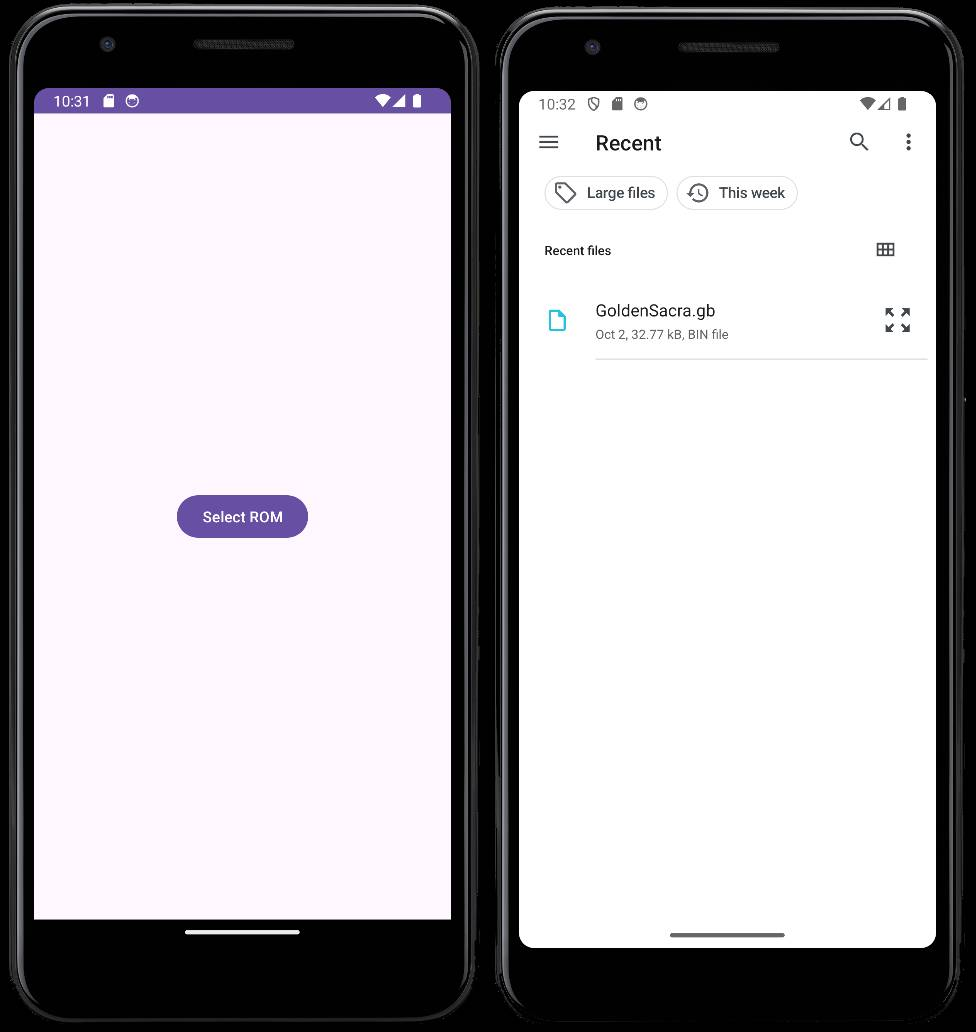
\includegraphics[width=0.4\textwidth]{include/images/openfile.jpg}
\caption{Selección de archivo desde la memoria SD del dispositivo.}
\label{figure:sdopen}
\end{figure}

A continuación, se procede a obtener los bytes del archivo y se envían al módulo de Emulator. En este momento, nos centraremos únicamente en la parte correspondiente a la ROM:

\begin{lstlisting}[language=Kotlin, caption={Carga de ROM y manejo de errores durante el proceso.}, label={code:kotlinloadrom}]
    fun load_rom(romBytes: ByteArray): Boolean{

        try {
            if(romBytes.isNotEmpty()){
                val cartSize = min(romBytes.size, ROM_END - ROM_START + 1)

                for (i in 0 until cartSize) {
                    Memory.write(ROM_START + i, romBytes[i])
                }

                return rom_init(romBytes)
            }
        }catch (ex: Exception){
            println("Error loading ROM: $ex")
        }

        return false
    }
\end{lstlisting}

En la función, se comprueba que los bytes pasados como parámetro no sean nulos. A continuación, se calcula el tamaño total de la ROM para asegurar que no exceda el tamaño máximo permitido (rango de 0x0000 a 0x7FFF). Se escriben todos los bytes en la memoria del emulador, y se invoca la función \textit{rom\_init()} para obtener datos como el título. Si alguna de las operaciones anteriores falla, se devuelve false y la ejecución se detiene.

\begin{lstlisting}[language=Kotlin, caption={Carga de ROM y manejo de errores durante el proceso.}, label={code:kotlinloadromread}]
    enum class CONSOLE_TYPE(val value : Int){
        DMG(0),
        DMG_CGB(0x80),
        CGB(0xC0),
        UNKNOWN(-1);

        companion object {
            fun fromValue(value: Int): CONSOLE_TYPE {
                return entries.find { it.value == value } ?: UNKNOWN
            }
        }
    }
    
    private var bootSection = ByteArray(0xFF)

    private var cartTitle : String      = "Unknown"
    private var licenseCode : String    = "None"
    private var cartType : Int          = -1
    private var romSize : Int           = -1
    private var ramSize : Int           = -1
    private var romVersion : Int        = -1
    private var console: CONSOLE_TYPE   = CONSOLE_TYPE.UNKNOWN

    [...]

    val newLicenseCodes: Map<String, String> = mapOf(
        "00" to "None",
        "01" to "Nintendo R&D1",
        "08" to "Capcom",
        "13" to "Electronic Arts",
        [...]
        "A4" to "Konami (Yu-Gi-Oh!)",
    )

    val oldLicenseCodes : Map<Int, String> = mapOf(
        0x00 to "None",
        0x01 to "Nintendo",
        0x08 to "Capcom",
        0x09 to "HOT-B",
        [...]
        0xFF to "LJN"
    )

    val cartTypes : Map<Int, String> = mapOf(
        0x00 to "ROM ONLY",
        0x01 to "MBC1",
        0x02 to "MBC1+RAM",
        0x03 to "MBC1+RAM+BATTERY",
        0x05 to "MBC2",
        [...]
        0xFF to "HuC1+RAM+BATTERY"
    )

    val ramSizes : Map<Int, Int> = mapOf(
        0x00 to 0, // KiB
        0x01 to 2,
        0x02 to 8,
        0x03 to 32,
        0x04 to 128,
        0x05 to 64
    )

    [...]

    fun convertBytesToString(bytes: ByteArray): String {
        val title = bytes.takeWhile { it != 0.toByte() && it.toInt() in 32..126 } // Filter only ASCII characters
        return String(title.toByteArray(), Charsets.US_ASCII)
    }

    fun rom_init(romBytes: ByteArray): Boolean{

        // Compare Cartridge Header with the Boot fixed one

        // Get header section from the romBytes
        val bootByteArray = Memory.getNintendoLogo()
        val cartByteArray = extractByteArray(romBytes, N_LOGO_START, N_LOGO_END, true) // Nintendo Logo on Cartridge goes from 0x104 to 0x133

        if(memcmp(Memory.getNintendoLogo(), cartByteArray, bootByteArray.size) != 0){
            return false
        }

        cartTitle   = convertBytesToString(extractByteArray(romBytes, TITLE_START, TITLE_END, true))

        licenseCode = if((extractByte(romBytes, OLD_LCNS_CODE).toInt() and 0xFF) == NEW_LICENSE_CODE){
            getNewLicenseNameFromIndex(convertBytesToString(extractByteArray(romBytes, LCNS_CODE_START, LCNS_CODE_END, true)))
        }else{
            getOldLicenseNameFromIndex(extractByte(romBytes, OLD_LCNS_CODE).toInt() and 0xFF)
        }

        cartType    = extractByte(romBytes, CART_TYPE).toInt() and 0xFF
        romSize     = 32 * (1 shl extractByte(romBytes, ROM_SIZE).toInt() and 0xFF) // Value in KiB
        ramSize     = extractByte(romBytes, RAM_SIZE).toInt() and 0xFF
        romVersion  = extractByte(romBytes, ROM_V_NUM).toInt() and 0xFF
        console     = CONSOLE_TYPE.fromValue(extractByte(romBytes, TITLE_END).toInt() and 0xFF)

        println("ROM Loaded Successfully!")

        bootSection = extractByteArray(romBytes, 0x00, 0xFF, true) // Save portion of code where the boot is going to load

        return true
    }
\end{lstlisting}

Desglosemos el código:

\begin{enumerate}
    \item Se compara el logotipo de Nintendo almacenado en el módulo de memoria con el presente en el cartucho. Si no coinciden, se procede a finalizar la ejecución del programa.
    \item Se obtienen los bytes correspondientes al título del juego y se convierten a una cadena de texto utilizando el conjunto de caracteres ASCII. Dado que la longitud del título depende de la versión del cartucho, se detendrá la lectura al encontrar el primer valor 0x00.
    \item Se extrae el código de licencia. Primero, se verifica si el valor antiguo contiene 0x33 para utilizar los nuevos códigos de licencia. De lo contrario, se empleará el listado antiguo. Ambos listados pueden definirse mediante un par de mapas (\textit{Maps}) para acceder rápidamente al valor correspondiente según el código obtenido.
    \item A continuación, se extraen de manera directa los valores correspondientes al tipo de cartucho, tamaño de la ROM/RAM, versión de la ROM y el tipo de mapper.
    \item Se realiza una copia de la región 0x0000-0x00FF del cartucho. La Game Boy "oculta" esta porción de código hasta que la secuencia de arranque ha finalizado.
\end{enumerate}

Aquí los resultados obtenidos con la carga de las ROMS \textit{Super Marioland}, \textit{Pokémon Azul} y \textit{Harry Potter y la Piedra Filosofal}:

\begin{lstlisting}[language=Consola, caption={Valores obtenidos tras la carga de ROM.}, label={code:romresults}]
--- Super Marioland
Cart Title: SUPER MARIOLAND
License: Nintendo
Cart Type: MBC1
ROM Size: 64
ROM Version Number: 0
RAM Size: 0
Console Type: DMG

--- Pokemon Azul
Cart Title: POKEMON BLUE
License: Nintendo R&D1
Cart Type: MBC5+RAM+BATTERY
ROM Size: 1024
ROM Version Number: 0
RAM Size: 3
Console Type: DMG

--- Harry Potter y la Piedra Filosofal
Cart Title: HARRYPOTTERBHVE
License: EA (Electronic Arts)
Cart Type: MBC5+RAM+BATTERY
ROM Size: 4096
ROM Version Number: 0
RAM Size: 2
Console Type: CGB
\end{lstlisting}

Además, se puede observar que la ROM se ha cargado correctamente en nuestra memoria virtual. En el caso de \textit{Harry Potter} y la piedra filosofal, los siguientes bytes son visibles en la región 0x0000-0x015F:

\begin{lstlisting}[language=Consola, caption={Visualización de la ROM cargada en la memoria virtual.}, label={code:rommemloaded}]
0000: E1 CD 9D 31 E9 87 87 87 85 6F 3E 00 8C 67 7E C9  | ...1.....o>..g~.
0010: 7A BC C0 7B BD C9 FF FF 3E 01 E0 A6 C9 FF FF FF  | z..{....>.......
0020: AF E0 A6 3E 02 E0 A8 C9 7C E0 51 7D E0 52 7A E0  | ...>....|.Q}.Rz.
0030: 53 7B E0 54 79 E0 55 C9 40 F5 D1 7B EA BA CD C9  | S{.Ty.U.@..{....
0040: C3 80 36 FF FF FF FF FF C3 CE C0 C3 AC 23 FF FF  | ..6..........#..
0050: FB C3 AC 39 FF FF FF FF C3 A3 38 FF FF FF FF FF  | ...9......8.....
0060: D9 D7 38 04 D5 54 5D E1 CB 2A CB 1B CB 2A CB 1B  | ..8..T]..*...*..
0070: CB 2A CB 1B 19 19 19 C9 CB 7C C8 F5 7D 2F C6 01  | .*.......|..}/..
0080: 6F 7C 2F CE 00 67 F1 C9 F5 79 2F C6 01 4F 78 2F  | o|/..g...y/..Ox/
0090: CE 00 47 F1 C9 CB 7A C8 F5 7B 2F C6 01 5F 7A 2F  | ..G...z..{/.._z/
00A0: CE 00 57 F1 C9 C5 06 08 AF 87 CB 15 30 04 84 30  | ..W.........0..0
00B0: 01 2C 05 20 F4 65 6F C1 C9 AF B5 20 03 65 37 C9  | .,. .eo.... .e7.
00C0: C5 D5 06 08 4D 2E 00 CB 14 CB 15 5D 7D 91 6F 3F  | ....M......]}.o?
00D0: 38 01 6B 05 20 F1 CB 14 B7 D1 C1 C9 C5 4D 44 3E  | 8.k. ........MD>
00E0: 0F 21 00 00 CB 23 CB 12 30 01 09 29 3D 20 F5 CB  | .!...#..0..)= ..
00F0: 7A 28 01 09 C1 C9 19 3E 02 EA 00 20 5E 23 56 C9  | z(.....>... ^#V.
0100: 00 C3 50 01 CE ED 66 66 CC 0D 00 0B 03 73 00 83  | ..P...ff.....s..
0110: 00 0C 00 0D 00 08 11 1F 88 89 00 0E DC CC 6E E6  | ..............n.
0120: DD DD D9 99 BB BB 67 63 6E 0E EC CC DD DC 99 9F  | ......gcn.......
0130: BB B9 33 3E 48 41 52 52 59 50 4F 54 54 45 52 42  | ..3>HARRYPOTTERB
0140: 48 56 45 C0 36 39 00 1B 07 02 01 33 00 D7 B4 78  | HVE.69.....3...x
0150: A7 FE 11 3E 00 20 01 3C E0 EF 31 FF CF F0 EF B7  | ...>. .<..1.....
\end{lstlisting}

\subsection{Lectura/Escritura en ROM}\label{rom:read_write}

\paragraph{Implementación de las Acciones de Lectura y Escritura en ROM}
Para implementar las operaciones, es necesario tener en cuenta cómo cada \hyperref[history_mbcs]{MBC} gestiona de manera específica las diferentes regiones de memoria y los registros asociados. Cada MBC presenta un mecanismo particular para el acceso y la selección de bancos de ROM y RAM, lo que afecta directamente la forma en que el emulador debe interactuar con ellos.
\\\\
Con el objetivo de lograr un emulador completo, es imprescindible implementar todos los tipos de controladores, desde el MBC1 hasta el MBC7, así como otros controladores especiales. No obstante, en este apartado se detallará exclusivamente la implementación del MBC1, que abarca una amplia gama de títulos, incluyendo juegos como \textit{Tetris DX} y \textit{Mario \& Yoshi}.
\\\\
La estructura propuesta, de forma que se faciliten la integración de los distintos tipos de MBC, es la siguiente:
\begin{itemize}
    \item Se generará una interfaz llamada MBCInterface, el cual tendrá dos funciones a implementar de lectura y escritura.
    \item Una clase abstracta MBC la cual implementa la interfaz y que contendrá datos como el modo de banca, el banco actual de ROM o los bancos de RAM.
    \item El módulo de ROM contendrá una variable de clase de tipo MBCInterface que por defecto será nulo y que obtendrá valor en la lectura inicial de ROM.
    \item El tipo NoMBC implementará directamente el MBCInterface, mientras que MBC1 heredará de la clase abstracta MBC.
    \item A la hora de escribir o leer en ROM, simplemente se trasladará la responsabilidad de la tarea a la variable guardada.
\end{itemize}

\begin{lstlisting}[language=Kotlin, caption={Inicialización del MBC.}, label={code:initmbc}]
    private var mbcInterface: MBCInterface?     = null
    [...]
    private fun initMBC(romBytes: ByteArray){
        mbcInterface = when(getCartTypeIndex()){
            0 -> NoMBC(romBytes)
            1 -> MBC1(romBytes)
            [...] // Resto de controladores
            else -> null
        }
    }   
\end{lstlisting}

Como ya ha sido explicado, dependiendo de las regiones de memoria en las que se intente escribir, se deben actualizar unos registros específicos.

\begin{lstlisting}[language=Kotlin, caption={Lectura en regiones ROM.}, label={code:romreadkotlin}]
    override fun read(address: Int): Byte {
        when (address) {
            in ROM_START..< ROM_SW_START -> { // READ FROM ROM FIXED BANK
                return when(bankingMode){
                    BankingMode.MODE_0 -> Memory.read(address)
                    BankingMode.MODE_1 -> romData?.get(getROM0BankAddr(address)) ?: 0xFF.toByte()
                }
            }
            in ROM_SW_START..ROM_END -> return romData?.get(getROMSwBankAddr(address)) ?: 0xFF.toByte() // READ FROM SWITCHABLE ROM BANK
            in EXTERNAL_RAM_START..< WRAM_START -> { // READ FROM EXTERNAL RAM
                return if(ramEnabled) {
                    ramBanks!![currentRamBank][address - EXTERNAL_RAM_START]
                } else 0xFF.toByte()
            }
        }

        return 0xFF.toByte()
    }
\end{lstlisting}

Desglosemos el código:

\begin{itemize}
    \item Si la dirección de memoria a leer se encuentra en el rango \texttt{0x0000-0x3FFF} (ROM fija o estática), primero se comprobará el modo de banco. En el caso del modo básico, la lectura se redirigirá al módulo de memoria. Para el modo avanzado, la lectura se realizará directamente sobre los bytes cargados del fichero \texttt{.gb/.gbc}. La función \texttt{getROM0BankAddr(address: Int)} verifica la cantidad de bancos ROM que contiene el cartucho, aplicando, si es necesario, una máscara y utilizando el registro de dos bits de la región \texttt{0x4000-0x5FFF} de manera complementaria.

    \item Si la dirección se encuentra en la región de ROM dinámica, \texttt{0x4000-0x7FFF}, los datos se obtendrán directamente del fichero \texttt{.gb/.gbc}. La función \texttt{getROMSwBankAddr(address: Int)} implementará una lógica similar a la de \texttt{getROM0BankAddr}, con la diferencia de que, en este caso, se sumará el resultado de la multiplicación entre el número de banco ROM actual y el tamaño de un banco (16 KiB) a la dirección indicada.

    \item Si la dirección se encuentra dentro del rango de la RAM externa, se comprobará primero que esta esté activada, para proceder a leer los valores correspondientes de la variable de clase.
\end{itemize}

Veamos ahora la escritura:

\begin{lstlisting}[language=Kotlin, caption={Escritura en regiones ROM.}, label={code:romwritekotlin}]
    override fun write(address: Int, value: Byte) {
        val valueInt = value.toInt() and 0xFF

        when {
            address <= ENABLE_RAM_END -> {  // ENABLE RAM
                if(cartHasRam())
                    ramEnabled = valueInt and 0xF == 0xA
            }
            address in (ENABLE_RAM_END + 1)..ROM_BANK_NUMBER_END -> {                           // ROM BANK SELECTION
                var currentRomBank = valueInt and romBankMask
                if (currentRomBank == 0) currentRomBank += 1
            }
            address in (ROM_BANK_NUMBER_END + 1)..RAM_BANK_NUMBER_END -> {                      // RAM BANK SELECTION
                if (bankingMode == BankingMode.MODE_1 && saveNeeded) {
                    saveExRAMToFile()
                }
                currentRamBank = valueInt and 0b11
            }
            address in (RAM_BANK_NUMBER_END + 1)..RAM_BANK_MODE_END -> {                        // BANKING MODE
                bankingMode = if (valueInt and 0b1 != 0) BankingMode.MODE_1 else BankingMode.MODE_0

                if(bankingMode == BankingMode.MODE_1 && saveNeeded){
                    saveExRAMToFile()
                }
            }
            address in EXTERNAL_RAM_START..< WRAM_START -> {                                       // WRITE TO EXTERNAL RAM
                if(ramEnabled){
                    ramBanks!![currentRamBank][address - EXTERNAL_RAM_START] = value

                    if(cartHasBattery()) saveNeeded = true
                }
            }
        }
    }
\end{lstlisting}

Desglosemos nuevamente el código:

\begin{itemize}
    \item Si la dirección de memoria se encuentra en el rango \texttt{0x0000} hasta \texttt{0x1FFF}, se realiza la habilitación de RAM externa. 
    \begin{itemize}
        \item Si el cartucho incluye RAM, se habilita la RAM cuando los 4 bits inferiores del valor escrito (\texttt{value}) son iguales a \texttt{0xA}.
    \end{itemize}
    
    \item Si la dirección está en el rango desde \texttt{0x2000} hasta \texttt{0x3FFF}, se selecciona el banco de ROM.
    \begin{itemize}
        \item Se determina el banco de ROM actual utilizando una máscara \texttt{romBankMask} y aplicándola a \texttt{value}. 
        \item Si el banco resultante es el banco 0 (que está reservado), se ajusta el valor a 1 para evitar acceder a la ROM reservada.
    \end{itemize}
    
    \item Si la dirección está en el rango desde \texttt{0x4000} hasta \texttt{0x5FFF}, se selecciona el banco de RAM.
    \begin{itemize}
        \item Si el modo de banca está en básico y es necesario guardar el estado, se llama a la función \texttt{saveExRAMToFile()} para almacenar los datos en el archivo de RAM externa.
    \end{itemize}
    
    \item Si la dirección está en el rango desde \texttt{0x6000} hasta \texttt{0x7FFF}, se define el modo de banca.
    \begin{itemize}
        \item Se selecciona el modo 1 si el bit menos significativo es 1, y modo 0 en caso contrario.
        \item Si el modo seleccionado es el básico y se requiere guardar, se realiza nuevamente el guardado con \texttt{saveExRAMToFile()}.
    \end{itemize}
    
    \item Si la dirección cae en el rango de RAM externa, \texttt{0xA000} hasta \texttt{0xBFFF}, se realiza una escritura en la RAM externa.
    \begin{itemize}
        \item Si la RAM está habilitada, el valor se escribe en el banco de RAM actual, ajustando la dirección para obtener la posición correcta.
        \item Si el cartucho tiene batería, se establece un flag para indicar que se requiere guardar.
    \end{itemize}
\end{itemize}

Con esto ya tendríamos lo básico para que nuestro controlador funcione. Partiendo de este ejemplo, se deben implementar el resto de los tipos existentes para asegurar que cualquier juego funcione.

\section{Interrupciones}

Las interrupciones deben ser procesadas en todos los ciclos de CPU, justo antes de ejecutar la siguiente instrucción de ROM. En la siguiente implementación, se puede ver el inicio del método \texttt{tick()}:

\begin{lstlisting}[language=Kotlin, caption={Interrupciones en el método principal de la CPU.}, label={code:cpuhandleinterrupt}]
    fun tick(): Boolean{

        // Interrupciones
        if(!pendingEI){
            handleInterrupts()
        }else{
            pendingEI = false
            Interrupt.enableInterrupts(true)
        }

        [...]
\end{lstlisting}

El flag \textit{pendingEI} es una variable que se activa en el momento que un opcode EI es ejecutado. Como se explicó previamente, esta instrucción no habilita las interrupciones de forma inmediata, si no que toma efecto en el siguiente ciclo de ejecución.
\\\\
En el método \texttt{handleInterrupts()}, se va a comprobar que las interrupciones estén habilitadas y que se deba procesar al menos una. En caso de que ambas condiciones se cumplan, se delegará el trabajo al módulo específico de las interrupciones.
\\\\
La lógica principal del módulo es la siguiente:

\begin{lstlisting}[language=Kotlin, caption={Lógica principal del módulo Interrupt.}, label={code:interruptlogic}]
    fun flush(){
        val activeInterrupts = getPendingInterrupts()

        if ((activeInterrupts and InterruptType.VBLANK.getInterruptMask()) != 0)        return handleInterrupt(VBLANK_PTR, InterruptType.VBLANK)
        else if ((activeInterrupts and InterruptType.LCD_STAT.getInterruptMask()) != 0) return handleInterrupt(LCD_STAT_PTR, InterruptType.LCD_STAT)
        else if ((activeInterrupts and InterruptType.TIMER.getInterruptMask()) != 0)    return handleInterrupt(TIMER_PTR, InterruptType.TIMER)
        else if ((activeInterrupts and InterruptType.SERIAL.getInterruptMask()) != 0)   return handleInterrupt(SERIAL_PTR, InterruptType.SERIAL)
        else if ((activeInterrupts and InterruptType.JOYPAD.getInterruptMask()) != 0)   return handleInterrupt(JOYPAD_PTR, InterruptType.JOYPAD)
    }

    private fun handleInterrupt(address: Int, type: InterruptType){
        enableInterrupts(false)       // IME se deshabilita para prevenir que otras interrupciones se ejecuten

        // Desactivar interrupciones
        val bit = (type.getInterruptMask()).inv()
        val ifValue = (Memory.getByteOnAddress(IF).toInt() and 0xFF)
        set_IF(ifValue and bit)

        CPU.executeInterrupt(address)
    }
\end{lstlisting}

Primero se ejecuta la función \texttt{flush()}, la cual se encarga de verificar las interrupciones pendientes y, si se detecta alguna, manejarla de manera adecuada:

\begin{enumerate}
    \item Se obtienen las interrupciones activas mediante la función getPendingInterrupts(), que retorna una máscara de bits representando las interrupciones pendientes.
    \item Se evalúa si cada tipo de interrupción está activa utilizando operaciones AND en combinación con las máscaras de interrupción.
    \item Si se detecta una interrupción activa para el tipo VBLANK, se llama a la función \texttt{handleInterrupt()} con la dirección de interrupción (0x0040) y el tipo correspondiente, finalizando así la ejecución de flush. Para el resto de tipos se hace lo mismo, siguiente la prioridad de bit.
\end{enumerate}

Por otro lado, la función \texttt{handleInterrupt(address: Int, type: InterruptType)} gestiona el proceso de atender una interrupción específica, asegurándose de que no se produzcan interrupciones adicionales durante su ejecución.

\begin{enumerate}
    \item Se deshabilitan las interrupciones globalmente llamando a enableInterrupts(false). Esto evita que otras interrupciones se ejecuten mientras se atiende la actual.
    \item Se lee el valor actual del registro IF, se realiza una operación bit a bit and con la máscara invertida para desactivar el bit correspondiente a la interrupción actual, y se actualiza en memoria.
    \item Finalmente, se ejecuta la rutina de servicio de interrupción llamando al método \\
    \texttt{executeInterrupt(address)}. En este se desactiva el HALT de la CPU (en caso de que lo estuviese), se pushea PC al stack pointer, y se sobreescribe PC con la dirección obtenida por parámetro. 
\end{enumerate}

Lo que ocurra a continuación depende de la decisión que haya tomado el desarrollador del juego que se ejecute.

\section{Temporizadores / Timers}

La implementación debe simular el comportamiento de los \hyperref[history_timer]{temporizadores} en el hardware original. Para ello se comenzará declarando unas constantes que representen las direcciones de memoria reales y se generarán las funciones de lectura y escritura:\label{writeToTimer}

\begin{lstlisting}[language=Kotlin, caption={Lectura y escritura en registros de Timers.}, label={code:timerwriteread}]
    const val DIV   = 0xFF04 // Divider Register (16 bit Register, but only the upper 8 bit (0-7) are public to the developer)
    const val TIMA  = 0xFF05 // Timer Counter
    const val TMA   = 0xFF06 // Timer Module
    const val TAC   = 0xFF07 // Timer Control

    [...]

    fun readFromTimer(address: Int): Byte{
        when(address){
            DIV -> return ((div16 shr 8) and 0xFF).toByte()
            TIMA -> return Memory.read(TIMA)
            TMA -> return Memory.read(TMA)
            TAC -> return Memory.read(TAC)
        }

        return 0
    }

    fun writeToTimer(address: Int, value: Byte){
        when(address){
            DIV -> {
                div16 = (div16 and 0xFF00)
            }
            TIMA -> Memory.write(TIMA, value)
            TMA -> Memory.write(TMA, value)
            TAC -> Memory.write(TAC, value)
        }
    }
\end{lstlisting}

A la hora de interactuar con el registro DIV, es importante considerar que internamente consta de 16 bits, aunque externamente solo se exponen los 8 bits más altos. Para manejarlo, se utiliza una variable de clase llamada \textit{div16}, que se inicializa siempre en 0x0000.
\\\\
Cuando se realiza una operación de escritura en este registro, únicamente se reinician a 0 los 8 bits menos significativos, preservando el estado de los 8 bits más altos. Por otro lado, al leer el registro, solo se devuelven los 8 bits más altos del valor contenido.
\\\\
Por último, se debe implementar la función que actualice en cada ciclo de ejecución el temporizador. Los pasos que debe seguir son:

\begin{itemize}
    \item Comparar el valor actual de DIV y verificar si ha llegado el momento de incrementar el contador TIMA basado en el valor de TAC (registro de control del temporizador).
    \item Usar el valor de TAC para determinar la frecuencia de incremento de DIV. Dependiendo de los dos primeros bits de TAC, el temporizador se incrementará a una velocidad diferente (256, 4, 16 o 64 ciclos de máquina).
    \item Si TIMA llega a 0xFF, se recarga con el valor de TMA y se genera una interrupción de temporizador.
\end{itemize}

\begin{lstlisting}[language=Kotlin, caption={Lectura y escritura en registros de Timers.}, label={code:timertick}]
    fun tick(){
        val prevDIV = div16
        div16 += 1

        var timerUpdate = false
        val tacValue = Memory.read(TAC).toInt() and 0xFF

        when(tacValue and 0b11){
            0b00 -> timerUpdate = (prevDIV and (1 shl 9) != 0) && (div16 and (1 shl 9) == 0)
            0b01 -> timerUpdate = (prevDIV and (1 shl 3) != 0) && (div16 and (1 shl 3) == 0)
            0b10 -> timerUpdate = (prevDIV and (1 shl 5) != 0) && (div16 and (1 shl 5) == 0)
            0b11 -> timerUpdate = (prevDIV and (1 shl 7) != 0) && (div16 and (1 shl 7) == 0)
        }

        if(timerUpdate && (tacValue and (1 shl 2) != 0)){
            var timaValue = Memory.read(TIMA).toInt() and 0xFF
            timaValue++
            Memory.write(TIMA, timaValue.toByte())

            if(timaValue == 0xFF){
                Memory.write(TIMA, Memory.read(TMA))
                Interrupt.requestInterrupt(Interrupt.InterruptType.TIMER.getByteMask())
            }
        }
    }
\end{lstlisting}

\section{RAM}

En la Game Boy, el término RAM puede hacer referencia a distintas áreas de memoria: WRAM (Working RAM), HRAM (High RAM), VRAM (Video RAM) o la RAM externa presente en algunos cartuchos. Este módulo se centrará en la implementación de WRAM y HRAM, ya que la VRAM está estrechamente vinculada al funcionamiento del módulo PPU (Processing Pixel Unit), mientras que la RAM externa está gestionada por los controladores de memoria de los cartuchos \hyperref[history_mbcs]{(MBC, Memory Bank Controllers)}.
\\\\
La implementación de la \textbf{HRAM}, siendo esta un espacio fijo de memoria, se delegará directamente al módulo Memory, que ya se encarga de manejar lecturas y escrituras en memoria. Debido a la simplicidad de su gestión y a que no requiere lógica específica adicional, no se desarrollará un apartado independiente para explicar su implementación en esta documentación.

\subsection{WRAM}
La WRAM en modo DMG es fija y se maneja directamente, mientras que en modo CGB incluye un banco fijo y hasta siete bancos conmutables adicionales, permitiendo que la memoria sea más dinámica. Estos bancos se almacenan en un array (\textit{wramBanks}) y el banco activo se controla mediante la variable \textit{wramBank}. Las lecturas y escrituras en la WRAM consideran si se está accediendo a un banco conmutable o al espacio fijo, ajustando automáticamente la dirección de memoria según sea necesario.

\begin{lstlisting}[language=Kotlin, caption={Lectura y escritura en Work RAM.}, label={code:wramreadwrite}]
    private var wramBanks: Array<ByteArray> = Array(CGB_SW_BANKS) { ByteArray(ECHO_RAM_START - SWITCHABLE_WRAM_START) } // Not used if not in CGB mode
    private var wramBank = 0

    fun readFromWRAM(address: Int) : Byte{
        return if(!ROM.isCGB() || address < SWITCHABLE_WRAM_START){
            Memory.read(address)
        }else{
            wramBanks[wramBank][address - SWITCHABLE_WRAM_START]
        }
    }

    fun writeToWRAM(address: Int, value: Byte){
        if(!ROM.isCGB() || address < SWITCHABLE_WRAM_START){
            Memory.write(address, value)
        }else{
            wramBanks[wramBank][address - SWITCHABLE_WRAM_START] = value
        }
    }
\end{lstlisting}

\subsection{VRAM}

Al estar estrechamente vinculada al módulo de la PPU, será ahi donde declaremos la variable. Únicamente se llegará a utilizar en modo CGB, ya que de otra forma acudiremos al módulo de memoria. Su implementación no tiene mucho más misterio: debe tener las dimensiones correctas y, en caso de estar en modo CGB, obtener o escribir los valores en ella:

\begin{lstlisting}[language=Kotlin, caption={Lectura y escritura en Video RAM.}, label={code:vramreadwrite}]
    private var vRam : ByteArray = ByteArray((VRAM_END - VRAM_START) + 1)

    fun readFromVRAM(address: Int) : Byte{
        return if(!ROM.isCGB()){
            Memory.read(address)
        }else{
            vRam[address - VRAM_START]
        }
    }

    fun writeToVRAM(address: Int, value: Byte){
        if(!ROM.isCGB()){
            Memory.write(address, value)
        }else{
            vRam[address - VRAM_START] = value
        }
    }
\end{lstlisting}

\subsection{RAM Externa}

La RAM Externa, como se ha visto, reside en los cartuchos y es gestionada por los controladores de memoria. En este caso, se ha implementado un controlador MBC1, por lo que la RAM externa se manejará a través de él. La lectura y escritura en la RAM externa se delegan al controlador MBC1, que se encarga de gestionar los bancos de RAM y de redirigir las operaciones a la RAM externa.
\\\\
La implementación ya se ha proporcionado en el apartado de \hyperref[rom:read_write]{lectura y escritura en ROM}.

\section{DMA}

Como se ha descrito en el \hyperref[dma]{apartado teórico}, definiremos una función que inicie el proceso de DMA. Por ahora no será utilizada, ya que para ello antes se debe implementar la PPU.
\\\\
En esta función de inicio daremos por activado el proceso, calcularemos la dirección de memoria sobre la que comenzar a iterar, y desactivaremos todas las interrupciones para que otra no pueda interrumpir la ejecución.

\begin{lstlisting}[language=Kotlin, caption={Inicio del proceso DMA.}, label={code:dmainit}]
    private var active : Boolean = false
    private var offset : Int = 0
    private var startAddress : Int = 0
    private var startDelay : Byte = 0

    fun start(value: Byte){ // Value: Indica el rango (0xXX00 - 0xXX9F)
        active = true
        offset = 0
        startDelay = 2
        startAddress = (value.toInt() and 0xFF) shl 8   // Si el valor es 0xC0, la dirección será 0xC000
        Interrupt.enableInterrupts(false) // Deshabilitamos las interrupciones
    }
\end{lstlisting}

En el método \textit{tick()} comprobaremos si hay o no un delay para comenzar la ejecución. En caso negativo obtendremos la dirección de inicio a la que le sumaremos el offset actual, y copiaremos el byte desde la RAM a la OAM. Al terminar de copiar los 160 bytes, desactivaremos el proceso y reactivaremos las interrupciones para continuar con la ejecución normal.

\begin{lstlisting}[language=Kotlin, caption={Proceso DMA.}, label={code:dmaprocess}]
    fun tick(){
        if (active){
            if(startDelay.toInt() == 0){
                val address = startAddress + offset
                PPU.writeToOAM(address, startAddress, Memory.getByteOnAddress(address))
                offset++
                active = (offset and 0xFF) < TOTAL_BYTES_TO_COPY

                if(!active)
                    Interrupt.enableInterrupts(true)
            }else{
                startDelay--
            }
        }
    }
\end{lstlisting}

\section{PPU}

En la PPU debemos antes de nada definir bastantes objetos con los que luego podamos trabajar de forma eficiente:
\begin{itemize}
    \item Enumeradores para obtener los bits individuales del LCDC, LCD Status, modo de PPU, paletas de color seleccionadas y atributos de un sprite.
    \item Un mapa que represente las distintas paletas y sus códigos de color con los que podamos trabajar en Android.
    \item Todas las variables de clase que necesitemos, como el contador de sprites por línea de renderizado, array de bytes para la VRam y la OAM, frame actual, paleta de color seleccionada, etc\ldots
\end{itemize}

Una vez definidos todos estos objetos, podremos pasar a inicializar la PPU:\label{handleLCDC}

\begin{lstlisting}[language=Kotlin, caption={Inicialización de la PPU.}, label={code:ppuinit}]
    fun init() {
        Memory.write(LCD_STAT, 0x81.toByte())
        Memory.write(LCDC_ADDR, 0x91.toByte())
        Memory.write(SCY, 0)
        Memory.write(SCX, 0)
        Memory.write(LY_ADDR, 0)
        Memory.write(LYC_ADDR, 0)
        Memory.write(WY, 0)
        Memory.write(WX, 0)
        val consoleType = ROM.getConsole()

        if(consoleType == ROM.CONSOLE_TYPE.DMG || consoleType == ROM.CONSOLE_TYPE.DMG_CGB) {
            Memory.write(BGP, 0xFC.toByte())
            Memory.write(OBP0, 0xFF.toByte())
            Memory.write(OBP1, 0xFF.toByte())
        }else{
            //TODO - CGB
        }

        handleLCDC(0x91.toByte())
    }

    [...]

    private fun handleLCDC(value: Byte){
        // Bit 7
        ppuEnabled = LCDCObj.LCDC_ENABLE.get(value) != 0
        lcdEnabled = ppuEnabled
        // Bit 6
        winTilemapAddr = if(LCDCObj.WIN_TILEMAP.get(value) == 0) TM_1_START else TM_2_START
        // Bit 5
        enabledWindow = LCDCObj.WINDOW_ENABLE.get(value) != 0
        // Bit 4
        addrModeAddr = if(LCDCObj.ADDRESS_MODE.get(value) == 0) SIGNED_TILE_REGION else VRAM_START
        // Bit 3
        bgTilemapAddr = if(LCDCObj.BG_TILEMAP.get(value) == 0) TM_1_START else TM_2_START
        // Bit 2
        objSize = if(LCDCObj.OBJ_SIZE.get(value) == 0) 8 else 16
        // Bit 1
        objEnabled = LCDCObj.OBJ_ENABLE.get(value) != 0
        // Bit 0
        bgWinEnabled = LCDCObj.MASTER_ENABLE.get(value) != 0
    }
\end{lstlisting}

Primero se configura la pantalla LCD:

\begin{itemize}
    \item \textbf{LCD Status (\texttt{LCD\_STAT})}: Se escribe el valor $0x81$ (\texttt{10000001} en binario). Este valor activa la interrupción cuando la línea de escaneo coincide con el valor de \texttt{LYC} y asegura que la pantalla empiece en un estado adecuado.
    \item \textbf{LCD Control (\texttt{LCDC})}: Se escribe el valor $0x91$ (\texttt{10010001} en binario), que habilita la pantalla, permite el uso de sprites y selecciona un modo de dirección de tiles.
\end{itemize}

Ahora configuramos los registros de desplazamiento y posición:
\begin{itemize}
    \item \textbf{\texttt{SCY} y \texttt{SCX}}: Se establecen en $0$ para que la imagen de fondo no esté desplazada.
    \item \textbf{\texttt{LY} y \texttt{LYC}}: Se inician en $0$ para que la pantalla empiece desde la primera línea de escaneo.
    \item \textbf{\texttt{WY} y \texttt{WX}}: Controlan la posición de la ventana en pantalla, comenzando en $0$.
\end{itemize}

Configuramos la paleta de colores detectando el tipo de consola:
\begin{itemize}
    \item Si es modo DMG o en en modo compatibilidad (DMG\_CGB):
    \begin{itemize}
        \item \textbf{\texttt{BGP}} se establece en $0xFC$ (\texttt{11111100} en binario), configurando la paleta de colores del fondo.
        \item \textbf{\texttt{OBP0} y \texttt{OBP1}} se establecen en $0xFF$, dejando los sprites con su configuración predeterminada.
    \end{itemize}
    \item Para el modo CGB, aún falta implementar la configuración específica.
\end{itemize}

Finalmente, se llama a \texttt{handleLCDC(0x91)} para aplicar la configuración del registro \texttt{LCDC}
\\\\
Al igual que el DMA y la CPU, la PPU también dispondrá de su propio método \texttt{tick()}. En él, comprobaremos que la PPU esté activa y ejecutaremos el código de los distintos modos según venga indicado en el \texttt{LCD Stat}.

\begin{lstlisting}[language=Kotlin, caption={Lógica principal de la PPU.}, label={code:pputick}]
    fun tick(){
        if(moduleIsActive()) {
            lineTicks++
            val stat = Memory.getByteOnAddress(LCD_STAT)

            when (StatObj.PPU_MODE.get(stat)) {
                PPUMode.HBlank.number -> hBlankMode(stat)       // MODE 0
                PPUMode.VBlank.number -> vBlankMode(stat)       // MODE 1
                PPUMode.OAM.number -> oamMode(stat)             // MODE 2
                PPUMode.DRAW_LCD.number -> drawLCDMode(stat)    // MODE 3
            }
        }
    }
\end{lstlisting}

\subsection{Modo 0: H-Blank}

El proceso verifica si se ha alcanzado el número total de ciclos (LINE\_TOTAL\_TICKS) para la línea actual y, si es así, se actualiza el valor del registro LY. Si la línea actual ha alcanzado o superado la resolución vertical de la Game Boy (GB\_Y\_RESOLUTION), significa que la PPU ha terminado de procesar todas las líneas visibles y entra en el modo V-Blank. En este caso, el método actualiza el estado de LCD\_STAT para reflejar este cambio y solicita una interrupción de V-Blank. Además, incrementa el contador de fotogramas y llama a calculateFPS() para actualizar la métrica de rendimiento.
\\\\
Por otro lado, si LY no ha alcanzado este límite, significa que la PPU aún está dentro del proceso de renderizado de la pantalla y debe volver al modo OAM. En este caso, el método actualiza LCD\_STAT para reflejar este cambio y, si la interrupción de estado del LCD para OAM está habilitada, solicita la interrupción correspondiente. Finalmente, restablece lineTicks a cero para comenzar el procesamiento de la nueva línea.

\begin{lstlisting}[language=Kotlin, caption={Lógica del proceso de H-Blank.}, label={code:ppuhblank}]
    private fun hBlankMode(stat: Byte){
        if(lineTicks >= LINE_TOTAL_TICKS){
            increment_LY()

            val ly = (Memory.getByteOnAddress(LY_ADDR).toInt()) and 0xFF

            if(ly >= GB_Y_RESOLUTION){ // ENTER VBLANK MODE
                Memory.write(LCD_STAT, StatObj.PPU_MODE.set(stat, PPUMode.VBlank.number))

                Interrupt.requestInterrupt(Interrupt.InterruptType.VBLANK.getByteMask()) // ASK FOR VBLANK INTERRUPT

                if(StatObj.VBLANK_INTERRUPT.get(stat) != 0)
                    Interrupt.requestInterrupt(Interrupt.InterruptType.LCD_STAT.getByteMask()) // ASK FOR LCD STAT INTERRUPT IF LCD_STAT HAS THE VBLANK BIT ACTIVATED

                currentFrame++

                calculateFPS()

            }else{ // RETURN TO OAM MODE
                Memory.write(LCD_STAT, StatObj.PPU_MODE.set(stat, PPUMode.OAM.number))

                if(StatObj.OAM_INTERRUPT.get(stat) != 0)
                    Interrupt.requestInterrupt(Interrupt.InterruptType.LCD_STAT.getByteMask()) // ASK FOR LCD STAT INTERRUPT IF LCD_STAT HAS THE OAM BIT ACTIVATED
            }

            lineTicks = 0
        }
    }
\end{lstlisting}

\subsection{Modo 1: V-Blank}

El proceso verifica si se ha alcanzado el número total de ciclos para la línea actual y, si es así, incrementa el valor del registro LY. Luego, obtiene el valor actualizado y comprueba si ha alcanzado o superado el número total de líneas. Si esto ocurre, significa que el periodo de V-Blank ha finalizado y la PPU debe volver al modo OAM para comenzar el renderizado del siguiente cuadro.
\\\\
En este caso, el método actualiza el estado de LCD\_STAT para reflejar el cambio al modo OAM y restablece LY\_ADDR a 0, indicando el inicio de un nuevo fotograma. Además, si la interrupción de estado del LCD para OAM está habilitada, solicita la interrupción. Al igual que en H-Blank, lineTicks se restablece a cero para comenzar el procesamiento de la nueva línea.

\begin{lstlisting}[language=Kotlin, caption={Lógica del proceso de V-Blank.}, label={code:ppuvblank}]
    private fun vBlankMode(stat: Byte){
        if(lineTicks >= LINE_TOTAL_TICKS){
            increment_LY()

            val ly = (Memory.getByteOnAddress(LY_ADDR).toInt()) and 0xFF

            if(ly >= TOTAL_LINES){ // RETURN TO OAM MODE
                Memory.write(LCD_STAT, StatObj.PPU_MODE.set(stat, PPUMode.OAM.number))
                Memory.write(LY_ADDR, 0)

                if(StatObj.OAM_INTERRUPT.get(stat) != 0)
                    Interrupt.requestInterrupt(Interrupt.InterruptType.LCD_STAT.getByteMask()) // ASK FOR LCD STAT INTERRUPT IF LCD_STAT HAS THE OAM BIT ACTIVATED
            }

            lineTicks = 0
        }
    }
\end{lstlisting}

\subsection{Modo 2: OAM Scan}

Aquí gestionamos el modo OAM Scan, el cual se encarga de escanear los sprites visibles en la línea actual antes de proceder al renderizado.
\\\\
Si el contador lineTicks ha alcanzado el número de ciclos necesarios para el modo OAM, la PPU cambia al modo de dibujo (DRAW\_LCD), actualizando el estado de LCD\_STAT y reiniciando los parámetros del FIFO fetcher, que se encarga de obtener los píxeles a renderizar. Sin embargo, en el primer ciclo, se inicializa el conteo de sprites en la línea y se llama a loadLineSprites(), que carga los sprites visibles en la línea actual para que puedan ser procesados durante la fase de dibujo.

\begin{lstlisting}[language=Kotlin, caption={Lógica del proceso de OAM Scan.}, label={code:ppuoamscan}]
    private fun oamMode(stat: Byte){ // MODE 2
        if(lineTicks >= OAM_CYCLES){ // ENTER DRAWING PIXELS MODE
            Memory.write(LCD_STAT, StatObj.PPU_MODE.set(stat, PPUMode.DRAW_LCD.number))
            fifoFetcher.resetParams() // Reset FIFO Fetcher
        }else if(lineTicks == 1){ // Scanning -> Read OAM on the first tick
            lineSpriteCount = 0
            loadLineSprites()
        }
    }
\end{lstlisting}

El método \texttt{loadLineSprites()} se encarga de seleccionar y ordenar los sprites que deben renderizarse en la línea de escaneo actual de la pantalla. Esta función solo se ejecuta si los sprites están habilitados o si la consola es un modelo CGB, ya que en este último caso siempre se procesan los sprites.
\\\\
Primero, se obtiene la línea de escaneo actual, sumándole un desplazamiento para compensar la posición real de los sprites. Luego, se determina el tamaño de los sprites, que puede ser de 8 o 16 píxeles. A continuación, se inicializa el array \texttt{objsFetched} con valores nulos y se resetea el contador que indica el número de sprites obtenidos por línea. Por último, se recorre la memoria OAM en bloques de 4 bytes (siendo cada uno en orden: posición Y, posición X, índice de tile y atributos). Si se han alcanzado el número máximo de sprites por línea, el bucle se detiene.
\\\\
Para cada sprite, se verifican las coordenadas x e y para determinar si es visible en la línea actual. Si lo es, se almacena en el array \texttt{objsFetched}, incrementando el contador a posteriori. Finalmente, se ordena la lista de sprites por su posición x, asegurando que aquellos con menor x se rendericen primero.

\begin{lstlisting}[language=Kotlin, caption={Obtención de sprites en modo OAM Scan.}, label={code:ppuoamscansprites}]
    private fun loadLineSprites(){

        if(objEnabled || ROM.isCGB()) { // CGB Ignores this condition

            val currentY = (Memory.getByteOnAddress(LY_ADDR).toInt() and 0xFF) + OAM_Y_OFFSET
            val lcdc = Memory.getByteOnAddress(LCDC_ADDR)
            val objSize = LCDCObj.OBJ_SIZE.get(lcdc)
            val spriteHeight = if (objSize == 0) 8 else 16

            objsFetched.fill(null)
            lineSpriteCount = 0

            for (i in oamRam.indices step 4) {

                if (lineSpriteCount >= MAX_OBJ_PER_SCANLINE) {
                    break
                }

                val y = oamRam[i].toInt() and 0xFF
                val x = oamRam[i + 1].toInt() and 0xFF
                val tile = oamRam[i + 2]
                val flags = oamRam[i + 3]

                if (x == 0 || x >= (GB_X_RESOLUTION + OAM_X_OFFSET)) { // Sprite not visible
                    continue
                }

                if (y <= currentY && (y + spriteHeight) > currentY) { // Sprite on current line
                    objsFetched[lineSpriteCount] = OAMObj(y.toByte(), x.toByte(), tile, flags)
                    lineSpriteCount++
                }
            }

            objsFetched.sortBy { it?.x ?: Byte.MAX_VALUE} // Sort by X position
        }
    }
\end{lstlisting}

\subsection{Modo 3: Drawing Pixels}

El modo de dibujo es el proceso en el que la PPU renderiza los píxeles en la pantalla. En este modo, se obtienen los datos de los tiles y se procesan para generar la imagen final. La función \texttt{drawLCDMode()} gestiona este proceso:

\begin{lstlisting}[language=Kotlin, caption={Dibujado de píxeles en Modo 3.}, label={code:ppuoamdrawpixels}]
    private fun drawLCDMode(stat: Byte){

        fifoFetcher.process()

        if(fifoFetcher.getPushedPixels() >= GB_X_RESOLUTION){ // ENTER HBLANK MODE

            fifoFetcher.clear()

            Memory.write(LCD_STAT, StatObj.PPU_MODE.set(stat, PPUMode.HBlank.number))

            if(StatObj.HBLANK_INTERRUPT.get(stat) != 0)
                Interrupt.requestInterrupt(Interrupt.InterruptType.LCD_STAT.getByteMask()) // ASK FOR LCD STAT INTERRUPT IF LCD_STAT HAS THE HBLANK BIT ACTIVATED
        }
    }
\end{lstlisting}

El código propio del FIFO vendrá documentado más adelante, pero por ahora se debe entender que su función es transferir la información de los píxeles al búfer de la pantalla. 
\\\\
Después del proceso, se comprueba que el número total de píxeles (correspondientes a la línea actual) que se han añadido sea mayor o igual a la resolución horizontal de la pantalla. Si estamos en este caso, reiniciaremos el proceso volviendo al modo H-Blank, y lanzando una interrupcion del Stat si estuviese activo.

\subsection{FIFO Fetcher}

Como viene definido en la parte teórica, la GB disponía de dos FIFO's, los cuales trabajan de manera independiente para transferir los píxeles de Background y Window por un lado, y los Sprites por otro. El proceso original finalizaba haciendo una mezcla de la información proporcionada por ambos.
\\\\
En este proyecto se va a utilizar una implementación algo más sencilla, tanto de implementar como de entender, basada en la guía de programación de \cite{lld}.
\\\\
Como variables de clase, se necesita guardar:

\begin{itemize} 
    \item Estado del fetcher (las distintas etapas del procesado).
    \item Coordenada X del tile en VRAM del que se está obteniendo información.
    \item Coordenada X del scanline que se va a dibujar.
    \item El propio FIFO, del cual se realizará una implementación propia.
    \item El búfer de video, que será un array de enteros, con un tamaño fijo equivalente a \texttt{Resolución\_Y * Resolución\_X}.
    \item Un array de 3 bytes donde se irá insertando información específica del tile sobre el que se trabajará.
    \item Un array de 3 objetos OAM (definido más adelante) se guardarán los metadatos de los sprites.
    \item Un array de 6 bytes que almacene los datos de píxeles crudos de los sprites.
    \item La coordenada Y de la línea actual sobre la que se deben procesar los tiles.
    \item Coordenadas globales X e Y en el mapa de tiles para determinar qué tile de VRAM debe ser obtenido y procesado.
\end{itemize}

La lógica principal de procesado se ha implementado de la siguiente manera:

\begin{lstlisting}[language=Kotlin, caption={Código principal del FIFO Fetcher.}, label={code:ppufifoprocess}]
    fun process(){
        val scx = Memory.getByteOnAddress(SCX).toInt() and 0xFF
        val scy = Memory.getByteOnAddress(SCY).toInt() and 0xFF
        val ly  = Memory.getByteOnAddress(LY_ADDR).toInt() and 0xFF

        mapY = scy + ly
        mapX = scx + fetchX
        tileY = (mapY % 8) * 2

        if(PPU.getLineTicks() % 2 == 0){
            fetch()
        }
        pushPixelsToBuffer() // Push pixels to pipeline
    }

    private fun fetch(){
        when(state){
            FetcherState.OBTAIN_TILE -> getTile()               // Fetch the current tile identification in the BG Tilemap
            FetcherState.LOW_DATA_TILE -> getTileLowData()      // Fetch the low byte of the tile
            FetcherState.HIGH_DATA_TILE -> getTileHighData()    // Fetch the high byte of the tile
            FetcherState.SLEEP -> sleepState()
            FetcherState.PUSH -> pushState()
        }
    }
\end{lstlisting}

En primer lugar, \texttt{process()} accede a los registros de memoria SCX, SCY y LY. Utilizando estos registros, calcula las coordenadas absolutas (mapX, mapY) en el espacio del mapa de tiles. Por ejemplo, \texttt{mapY = SCY + LY} permite ajustar la renderización vertical según el desplazamiento del fondo, mientras que \texttt{mapX = SCX + fetchX} hace lo mismo para el eje horizontal. La variable tileY se deriva de \texttt{mapY \% 8} para identificar la línea específica dentro del tile actual, esencial para acceder a los datos de píxeles correctos en VRAM.
\\\\
Para evitar conflictos con el PPU, en la función se verifica el estado de los ciclos de renderizado mediante \texttt{PPU.getLineTicks() \% 2 == 0}. Esta condición asegura que \texttt{fetch()} solo se ejecute cada 2 ciclos de máquina, simulando el comportamiento del hardware real, donde el acceso a VRAM está restringido durante ciertas fases del renderizado.
\\\\
Finalmente, \texttt{pushPixelsToBuffer()} transfiere los píxeles desde el FIFO al búfer de video. Esta etapa es crítica para mantener un flujo constante de datos hacia la pantalla, asegurando que no haya retrasos en la visualización.
\\\\
La función \texttt{fetch()} implementa una máquina de estados, en el que cada estado representa una etapa específica del pipeline. Los estados son los siguientes:

\begin{itemize}
    \item \textbf{\texttt{OBTAIN\_TILE}}: donde se determina qué tile debe ser renderizado.
    \item \textbf{\texttt{LOW\_DATA\_TILE}}: donde se obtienen los datos de píxeles bajos del tile.
    \item \textbf{\texttt{HIGH\_DATA\_TILE}}: donde se obtienen los datos de píxeles altos del tile.
    \item \textbf{\texttt{SLEEP}}: donde se espera a que el ciclo de renderizado esté listo para continuar.
    \item \textbf{\texttt{PUSH}}: donde se transfieren los píxeles al búfer de video.
\end{itemize}

\subsubsection{OBTAIN\_TILE}
El fetcher determina el tile que debe ser renderizado. Accede al mapa de tiles (ubicado en \$9800-\$9BFF o \$9C00-\$9FFF, dependiendo de los flags del registro LCDC) para leer el índice del tile correspondiente a las coordenadas mapX y mapY. Este acceso a memoria es fundamental, ya que define los datos que se procesarán en los estados siguientes.

\begin{lstlisting}[language=Kotlin, caption={FIFO Fetcher - Obtención de Tile.}, label={code:ppufifogettile}]
    private fun getTile(){
        if(PPU.lcdIsEnabled())
            getBGTile()

        if(PPU.objsAreEnabled() && PPU.getFetchedSpriteEntries().isNotEmpty()) {
            fetchedSprites = 0
            getSpriteTile()
        }

        state = FetcherState.LOW_DATA_TILE
        fetchX += 8
    }
\end{lstlisting}

En primer lugar, la función \texttt{getBGTile()} realiza una lectura de los registros que controlan el desplazamiento y posicionamiento de los elementos gráficos. Estos incluyen el LY, las coordenadas de la ventana (WY y WX) y los valores de scroll (SCX y SCY).
\\\\
Posteriormente, la función realiza una evaluación de las posiciones relativas y los estados de los flags de control, para establecer si el tile que está siendo procesado pertenece al Background o al Window. Esta distinción determina qué tilemap debe ser consultado, alternando entre las zonas reservadas \texttt{0x9800} y \texttt{0x9C00} según corresponda.

\begin{lstlisting}[language=Kotlin, caption={FIFO Fetcher - Obtención de Tile de Background.}, label={code:ppufifogettilebg}]
    private fun getBGTile(){
        val ly = Memory.getByteOnAddress(LY_ADDR).toInt() and 0xFF
        val wy = Memory.getByteOnAddress(WY).toInt() and 0xFF
        val scx = Memory.getByteOnAddress(SCX).toInt() and 0xFF
        val wx = Memory.getByteOnAddress(WX).toInt() and 0xFF - WIN_X_OFFSET

        // Obtain tilemap to use (BG or WIN)
        val windowTile = isWindowTile()
        val tilemapToUse = if(windowTile) PPU.getWinTilemapAddr() else PPU.getBGTilemapAddr()

        val xCoordinate = if (windowTile) ((fetchX - wx) / 8) else (mapX / 8) and 0x1F
        val yCoordinate = if (windowTile) ((ly - wy) / 8) else (mapY / 8)

        val address = tilemapToUse + ((xCoordinate + (yCoordinate * GB_X_TOTAL_TILES)) and 0x3ff)
        var tile = Memory.getByteOnAddress(address) // 1 Tile == 8 Pixels

        if(PPU.getAddrModeAddr() == SIGNED_TILE_REGION){
            tile = ((tile.toInt() and 0xFF) + 128).toByte() // Signed Region [-128, 128] --> Transform to [0, 255]
        }
        tileData[0] = tile
    }
\end{lstlisting}

Se transforman las coordenadas globales, expresadas en píxeles, en índices específicos de tiles, teniendo en cuenta que cada elemento gráfico ocupa un área de 8x8 píxeles. Este cálculo considera tanto la posición absoluta en pantalla como también la incorporación de los efectos de desplazamiento producidos por el scroll.
\\\\
Si el modo de direccionamiento de tiles indica que se trata de una región con direcciones firmadas (índices que pueden ir de -128 a +127), se ajusta el valor sumándole 128 para convertirlo a un índice positivo válido. El identificador final del tile se guarda en el array \texttt{tileData}, dejándolo listo para ser usado en la siguiente fase.
\\\\
Por otro lado, la función \texttt{getSpriteTile()} se encarga de obtener el índice del tile correspondiente a los sprites visibles en la línea actual. Esta función es similar a la anterior, pero se centra en los sprites y su posición relativa en la pantalla.

\begin{lstlisting}[language=Kotlin, caption={FIFO Fetcher - Obtención de Tile de Sprites.}, label={code:ppufifogettileobj}]
    private fun getSpriteTile(){

        val fetchedObjs = PPU.getFetchedSpriteEntries()

        for (obj in fetchedObjs) {
            if(obj != null) {
                val scx = Memory.getByteOnAddress(SCX).toInt() and 0xFF
                val sprX = ((obj.x.toInt() and 0xFF) - OAM_X_OFFSET) + (scx % PIXELS_PER_TILE)

                if ((sprX >= fetchX && sprX < fetchX + OAM_X_OFFSET) ||
                ((sprX + OAM_X_OFFSET) >= fetchX && (sprX + OAM_X_OFFSET) < fetchX + OAM_X_OFFSET)) {
                    objTileData[fetchedSprites] = obj
                    fetchedSprites++
                }

                if (fetchedSprites >= 3) break
            }
        }
    }
\end{lstlisting}

La función recorre la lista proporcionada por la PPU \texttt{PPU.getFetchedSpriteEntries()} y comprueba, para cada sprite no nulo, su posición horizontal en pantalla. Para ello, obtiene el valor \texttt{SCX} desde memoria, y calcula la posición horizontal del sprite ajustando el valor original del sprite en el OAM, restando una constante que representa el desfase de coordenadas (\texttt{OAM\_X\_OFFSET}) y sumando un pequeño ajuste basado en el módulo del desplazamiento.
\\\\
Con la posición horizontal calculada, se evalúa si dicho sprite se encuentra dentro del rango de píxeles que se están a punto de dibujar, comparándolo con \texttt{fetchX}. Se realiza una doble condición para cubrir tanto la coincidencia exacta como los solapes de píxeles con el ancho de un sprite. Si el sprite cumple estas condiciones de visibilidad, se almacena en el array \texttt{objTileData}, y se incrementa el contador \texttt{fetchedSprites} que indica el número de sprites seleccionados.
\\\\
Este proceso continúa hasta que se han encontrado tres sprites coincidentes, momento en el cual el bucle se interrumpe. Esta limitación viene explicada en \hyperref[mem:oam]{el marco teórico}.

\subsubsection{LOW\_DATA\_TILE - HIGH\_DATA\_TILE}

En ambas funciones lo perimero que se realiza es el cálculo del offset vertical dentro del tile. Posteriormente, se accede a la VRAM para recuperar el primer o el segundo byte de datos de línea de ese tile, lo que representa los bits bajos o altos de color para los 8 píxeles de esa fila, respectivamente.
\\\\
La dirección a la que accede se compone usando el identificador del tile, el modo de direccionamiento actual, y la posición vertical dentro del tile. Una vez obtenido ese primer byte, se llama a \texttt{loadSpriteData()} con el desplazamiento correspondiente, para que se vayan cargando también los datos de los sprites superpuestos. Finalmente, se cambia el estado del fetcher al siguiente paso, \texttt{HIGH\_DATA\_TILE} o \texttt{SLEEP}, dependiendo del estado actual en el que se encuentre el fetcher.

\begin{lstlisting}[language=Kotlin, caption={FIFO Fetcher - Obtención de los Bits Bajos o Altos del Tile.}, label={code:ppufifogethighlowdata}]
    private fun getTileLowData(){
        val offset = calculeTileDataOffset()
        tileData[1] = Memory.getByteOnAddress(PPU.getAddrModeAddr() + ((tileData[0].toInt() and 0xFF) * 16) + offset)
        loadSpriteData(0)
        state = FetcherState.HIGH_DATA_TILE
    }

    private fun getTileHighData(){
        val offset = calculeTileDataOffset()
        tileData[2] = Memory.getByteOnAddress(PPU.getAddrModeAddr() + ((tileData[0].toInt() and 0xFF) * 16) + (offset + 1))
        loadSpriteData(1)
        state = FetcherState.SLEEP
    }
\end{lstlisting}

Finalmente, \texttt{loadSpriteData()} es la función auxiliar que realiza la lectura de los datos gráficos de los sprites que se van a dibujar sobre la línea actual. Por cada sprite, se calcula la línea dentro del tile que corresponde al valor actual de LY, considerando si el sprite está volteado verticalmente. También se ajusta el índice del tile en caso de sprites de 16 píxeles. Luego, se accede a VRAM para obtener el byte correspondiente a esa línea de píxeles dentro del tile del sprite, y se guarda en el bufer \texttt{objFetchedData}.
\\\\
Es una de las funciones que deberían estar separadas en una lógica independiente, pero que por eliminar cierta complejidad se ha incluido en lo que sería el fetcher de background.

\begin{lstlisting}[language=Kotlin, caption={FIFO Fetcher - Obtención de Información de un Sprite en la Línea Actual.}, label={code:ppufifogethighlowdatasprite}]
    private fun loadSpriteData(offset: Int){
        val ly = Memory.getByteOnAddress(LY_ADDR).toInt() and 0xFF
        val spriteHeight = if (LCDCObj.OBJ_SIZE.get(Memory.getByteOnAddress(LCDC_ADDR)) == 1) 16 else 8

        for(i in 0 until fetchedSprites){
            if(objTileData[i] != null) {
                val flags = objTileData[i]!!.flags
                val spriteY = (objTileData[i]!!.y.toInt() and 0xFF) - OAM_Y_OFFSET
                var tileIndex = objTileData[i]!!.tile.toInt() and 0xFF

                if (spriteHeight == 16)
                    if ((ObjFlags.Y_FLIP.get(flags) == 0 && (ly - spriteY) >= 8) ||
                        (ObjFlags.Y_FLIP.get(flags) == 1 && (ly - spriteY) < 8)) {
                        tileIndex += 1
                    }

                val baseAddress = VRAM_START + (tileIndex * 16)
                val tileLine = (ly - spriteY) % 8
                val address = baseAddress + (tileLine * 2)

                objFetchedData[(i * 2) + offset] = Memory.getByteOnAddress(address + offset)
            }
        }
    }
\end{lstlisting}

\subsubsection{SLEEP}
La implementación del estado \texttt{SLEEP} no va a tener nada relevante, simplemente va a dar paso al siguiente estado. Este método se utiliza para simular y representar los tiempos reales del hardware.

\begin{lstlisting}[language=Kotlin, caption={FIFO Fetcher - Sleep.}, label={code:ppufifosleep}]
    private fun sleepState(){
        state = FetcherState.PUSH
    }
\end{lstlisting}

\subsubsection{PUSH}

En la función \texttt{pushState()} se intenta introducir nuevos píxeles en el FIFO. Si el intento de empujar píxeles al FIFO tiene éxito (lo que significa que la cola tiene espacio suficiente), el estado del fetcher se reinicia para comenzar la obtención del siguiente tile.

\begin{lstlisting}[language=Kotlin, caption={FIFO Fetcher - Push.}, label={code:ppufifopush}]
    private fun pushState(){
        val bgPush = pushBGPixelsToFifo()

        if(bgPush){
            state = FetcherState.OBTAIN_TILE
        }
    }
\end{lstlisting}

La lógica principal ocurre en \texttt{pushBGPixelsToFifo()}, que primero comprueba si el FIFO tiene suficiente espacio libre para recibir una nueva tanda de píxeles, que son ocho por cada tile. Si está lleno, simplemente se detiene y devuelve false, esperando a que se vacíe en futuras iteraciones.
\\\\
Si hay espacio, la función calcula la posición horizontal real de dibujo teniendo en cuenta el SCX y una corrección por el offset de los sprites. A continuación, se procesan los píxeles del tile que acaba de ser cargado. Para cada uno, se extraen los bits correspondientes desde los datos de tile almacenados previamente en \texttt{objTileData}, combinando los bits bajos y altos de cada línea para determinar el índice de color del píxel.
\\\\
Este índice puede cambiar si los sprites están habilitados en la configuración del sistema. En tal caso, se llama a \texttt{obtainSpriteColor}, que se encarga de comprobar si algún sprite visible debe sobrescribir el color de fondo en esa posición. Esta función recorre los sprites previamente extraídos para el scanline actual y, si alguno se solapa con la posición del píxel en cuestión, evalúa si el sprite tiene prioridad sobre el fondo. También tiene en cuenta atributos como la inversión horizontal y la transparencia. Si se cumplen las condiciones, el color del sprite sobrescribe el del fondo.
\\\\
Nuevamente, esta última parte donde se obtienen los valores de los sprites y se hace una mezcla de valores para determinar el color, debería estar de forma independiente y ser añadido a un segundo FIFO.
\\\\
Por último se inserta el color en el FIFO de fondo, que es lo que usará el PPU para representar visualmente los píxeles en pantalla. Esto se repite para los ocho píxeles del tile, tras lo cual el método finaliza con éxito

\begin{lstlisting}[language=Kotlin, caption={FIFO Fetcher - Push de Píxeles al FIFO.}, label={code:ppufifopushpixels}]
    private fun pushBGPixelsToFifo(): Boolean{
        if(backgroundFifo.getSize() >= 8)
            return false // Fifo is full

        val scx = Memory.getByteOnAddress(SCX).toInt() and 0xFF
        val x = fetchX - (OAM_X_OFFSET - (scx % PIXELS_PER_TILE))

        for(i in 0..7){
            val bit = 7 - i

            val low = (((tileData[1].toInt() and 0xFF) shr bit) and 1)
            val high = ((((tileData[2].toInt() and 0xFF) shr bit) and 1) shl 1)
            var color = if(PPU.bgWinIsEnabled()) PPU.getColorIndex(high or low) else PPU.getColorIndex(0) // Pixel Color

            if(PPU.objsAreEnabled())
                color = obtainSpriteColor(color)

            if(x >= 0){
                backgroundFifo.push(color)
                fifoX++
            }
        }

        return true
    }
\end{lstlisting}

Los colores vienen definidos como propiedad de clase en la PPU, tratando de simular todas las posibles paletas de color que existen tanto en la GB original como en la CGB. Por defecto, se iniciará con la paleta que imita los colores verdosos del primer modelo DMG.

\begin{lstlisting}[language=Kotlin, caption={PPU - Paletas de Color.}, label={code:ppucolorpalettes}]
    // Colors follows as: White - Light Gray - Dark Gray - Black
    private val palettes: HashMap<PALETTE_TYPE, IntArray> = hashMapOf(
        Pair(PALETTE_TYPE.BASIC_PL, intArrayOf(0xFFFFFFFF.toInt(), 0xFFAAAAAA.toInt(), 0xFF555555.toInt(), 0xFF000000.toInt())),
        Pair(PALETTE_TYPE.GREENER_PL, intArrayOf(0xFFE0F8D0.toInt(), 0xFF88C070.toInt(), 0xFF346856.toInt(), 0xFF081820.toInt())),
        [...]
    )

    private var selectedPalette = PALETTE_TYPE.GREENER_PL
\end{lstlisting}

\section{Game Surface View}

El \texttt{GameSurfaceView} es la clase encargada de gestionar la representación gráfica de la consola. Esta clase se encarga de crear un canvas y dibujar los píxeles en él, utilizando el búfer de video proporcionado por la PPU. La implementación de esta clase es bastante sencilla, ya que solo se encarga de crear un canvas y dibujar los píxeles en él.
\\\\
La clase hereda de \texttt{SurfaceView} y está diseñada para funcionar de forma independiente gracias a un hilo (\texttt{GameThread}) que se encarga del renderizado continuo. Además implementa \texttt{SurfaceHolder.Callback}, lo cual permite controlar cuándo se crea, cambia o destruye el canvas.

\begin{lstlisting}[language=Kotlin, caption={Creación del Game Surface View.}, label={code:surfaceview}]
    class GameSurfaceView @JvmOverloads constructor(
        context: Context,
        attrs: AttributeSet? = null
    ) : SurfaceView(context, attrs), SurfaceHolder.Callback {

        private var scale : Float = 0f
        var debugMode = false
        private var gameThread: GameThread? = null

        init {
            holder.addCallback(this)
            gameThread = GameThread(holder, this)
        }

        [...]

\end{lstlisting}

El método \texttt{onMeasure()} se encarga de calcular las dimensiones basándose en la resolución original de la GB (160x144 píxeles) y en el tamaño disponible en pantalla. La idea es mantener la relación de aspecto original sin deformar la imagen. En función del ancho y alto del dispositivo, se calcula un factor de escala que se utilizará para transformar los píxeles al tamaño físico del dispositivo Android.

\begin{lstlisting}[language=Kotlin, caption={Medición y Escalado del Canvas.}, label={code:surfaceonmeasure}]
    override fun onMeasure(widthMeasureSpec: Int, heightMeasureSpec: Int) {
        val width = MeasureSpec.getSize(widthMeasureSpec) // Android phone total width
        val height = MeasureSpec.getSize(heightMeasureSpec)  // Android phone total height

        val aspectRatio = GB_X_RESOLUTION.toFloat() / GB_Y_RESOLUTION.toFloat() // GB Aspect Ratio

        val newWidth: Int
        val newHeight: Int

        if (width / height > aspectRatio) { // Landscape
            newWidth = (height * aspectRatio).toInt()
            newHeight = height
            scale = height / GB_Y_RESOLUTION.toFloat()
        } else { // Straight
            newWidth = width
            newHeight = (width / aspectRatio).toInt()
            scale = width / GB_X_RESOLUTION.toFloat()
        }

        setMeasuredDimension(newWidth, newHeight)
    }
    
\end{lstlisting}

Durante el renderizado, el método \texttt{render()} decide si debe dibujarse el bufer final donde la PPU guarda los colores o si se debe entrar en el modo depuración en el que se muestran los tiles disponibles en memoria. Si el LCD está deshabilitado, simplemente se pinta la pantalla de negro.
\\\\
Cuando se renderiza la VRAM, se recorre la matriz de píxeles que la PPU ha rellenado y se dibujan los píxeles uno por uno. Para cada tile, se leen 16 bytes de memoria. A partir de estos bytes, se reconstruye el color de cada píxel del tile utilizando la lógica de combinación de bits, y se pinta como un pequeño rectángulo en el canvas.

\begin{lstlisting}[language=Kotlin, caption={Medición y Escalado del Canvas.}, label={code:surfaceonmeasure}]
    private fun renderVRam(canvas: Canvas){
        val paint = Paint()

        for (lineNum in 0 until GB_Y_RESOLUTION) {
            for (x in 0 until GB_X_RESOLUTION) {
                val left = Math.round(x * scale).toFloat()
                val top = Math.round(lineNum * scale).toFloat()
                val right = left + ceil(scale.toDouble()).toFloat()
                val bottom = top + ceil(scale.toDouble()).toFloat()

                val color = PPU.getBufferPixelFromIndex(x + (lineNum * GB_X_RESOLUTION))
                paint.color = color

                canvas.drawRect(left, top, right, bottom, paint)
            }
        }
    }
    
\end{lstlisting}

Por último, el \texttt{GameThread} estará constantemente renderizando mientras que el flag \texttt{running} esté activado. Para hacer este render, primero bloquea el Canvas para ejecutar el método de renderizado del \texttt{GameSurfaceView} y finalmente libera el Canvas para que el sistema lo dibuje en pantalla.

\begin{lstlisting}[language=Kotlin, caption={Renderizado en el GameThread.}, label={code:surfacerenderthread}]
    override fun run() {
        while (running) {
            var canvas: Canvas? = null
            try {
                canvas = surfaceHolder.lockCanvas()
                if (canvas != null) {
                    synchronized(surfaceHolder) {
                        gameSurfaceView.render(canvas)
                    }
                }
            }catch (ex: Exception){
                ex.printStackTrace()
            } finally {
                if (canvas != null) {
                    surfaceHolder.unlockCanvasAndPost(canvas)
                }
            }
        }
    }
\end{lstlisting}

\subsection{Layout}

Ahora el EmuActivity contendrá el \texttt{GameSurfaceView} como variable privada de clase. Para hacerlo funcionar, se necesita también añadir la vista al layout y enlazarla con la variable en el \texttt{onCreate()}. Se puede insertar, por ejemplo, dentro de un \texttt{FrameLayout}:

\begin{lstlisting}[language=Kotlin, caption={GameSurfaceView en Layout.}, label={code:surfacelayout}]
    <FrameLayout
        android:id="@+id/frameLayout"
        app:layout_constraintTop_toTopOf="parent"
        app:layout_constraintStart_toStartOf="parent"
        app:layout_constraintEnd_toEndOf="parent"
        android:layout_width="match_parent"
        android:layout_centerInParent="true"
        android:padding="16dp"
        android:layout_height="wrap_content" >

        <es.atm.gbee.views.GameSurfaceView
            android:id="@+id/gameSurface"
            android:layout_width="wrap_content"
            android:layout_height="wrap_content"
            app:layout_constraintTop_toTopOf="parent"
            app:layout_constraintStart_toStartOf="parent"
            app:layout_constraintEnd_toEndOf="parent"
            />
    </FrameLayout>
\end{lstlisting}

De manera automática, se puede comenzar a ver resultados por pantalla. Aquí distintos resultados obtenidos según se han ido depurando errores, ordenados de forma cronológica:

\begin{figure}[H]
    \centering
    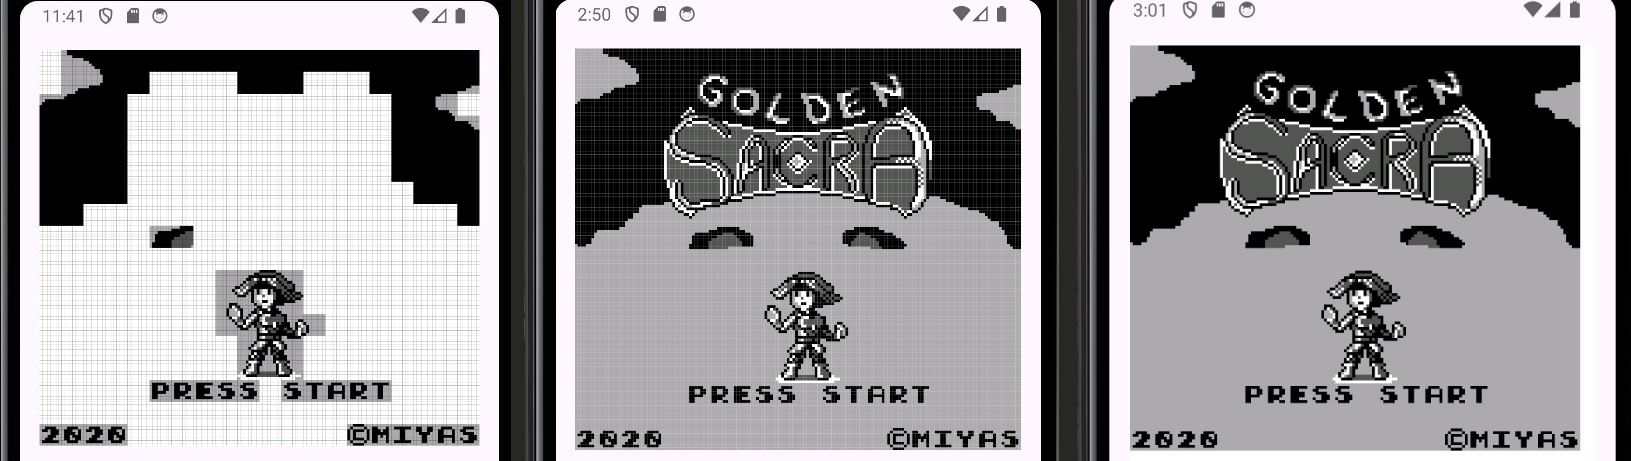
\includegraphics[width=1\textwidth]{include/images/render_surface_view.png}
    \caption{Renderizado de Tiles en SurfaceView}\label{figure:surface_view}
\end{figure}

\section{I/O}

Al igual que con el resto de módulos, se debe implementar el encargado de escribir y leer los registros de entrada y salida. Se definirán también un enumerador que indique a qué bit va asignado cada botón del joypad y un objeto que facilite hacer un seguimiento de cuáles están pulsados.

\begin{lstlisting}[language=Kotlin, caption={Estados de los Botones en el Módulo IO.}, label={code:iojoypad}]
    enum class GamePadBits(val bit: Int) {
        A_BUTTON(0),
        RIGHT_PAD(0),
        B_BUTTON(1),
        LEFT_PAD(1),
        SELECT_BUTTON(2),
        UP_PAD(2),
        START_BUTTON(3),
        DOWN_PAD(3),
        SELECT_DPAD(4),
        SELECT_BUTTONS(5);

        fun get(value: Byte): Int {
            return (value.toInt() and 0xFF) and (0b1 shl bit)
        }
    }

    object IO {

        private var serialData = ByteArray(2)

        data class GamepadState(
            var start: Boolean = false,
            var select: Boolean = false,
            var a: Boolean = false,
            var b: Boolean = false,
            var up: Boolean = false,
            var down: Boolean = false,
            var left: Boolean = false,
            var right: Boolean = false
        )

        private val gamePadState = GamepadState()

        [...]
\end{lstlisting}

Los métodos de lectura y escritura son muy similares al resto de módulos que ya se han explicado previamente, por lo que se van a omitir en esta explicación para evitar redundancias. Los puntos que se deben tener en cuenta son:

\begin{itemize}
    \item Si se escribe en el rango [0xFF40\-0xFF40], se delega a la PPU su comportamiento. En general, los casos especiales serán el inicio del DMA o cambios de \hyperref[handleLCDC]{comportamiento en el LCDC}.
    \item Si se escribe en el rango [0xFF04\-0xFF07], se delega al Timer su comportamiento, el cual ya se ha visto en su \hyperref[writeToTimer]{apartado correspondiente}.
\end{itemize}

El caso importante que se debe controlar en el propio módulo, es el del Joypad. La lógica a seguir es la siguiente:

\begin{enumerate}
    \item El \texttt{EmuActivity} indica que el jugador ha pulsado o dejado de pulsar un botón definido en el layout.
    \item Se actualiza la propiedad de la variable de clase con el nuevo valor.
    \item Se actualiza el valor en la memoria interna del emulador teniendo en cuenta el funcionamiento matricial original.
\end{enumerate}

A la hora de leer el joypad, simplemente se devuelve el valor almacenado en la memoria interna.
\\\\
En cuanto a la escritura, la función \texttt{updateJoyPadReadOnlyValues(value: Byte)} es el principal encargado. Empieza extrayendo los bits 4 y 5 del valor de entrada; estos bits indican qué grupo de botones se quiere consultar: los botones de dirección (arriba, abajo, izquierda, derecha) o los botones de acción (A, B, Start, Select). Esta selección se hace a través de los bits \texttt{SELECT\_DPAD} y \texttt{SELECT\_BUTTONS}.
\\\\
Si ambos selectores son iguales, no se selecciona ningún grupo concreto, y se ponen todos los bits de botones como "no presionados".
\\\\
Si solo uno de los dos selectores está activo, se determina cuál y se leen los estados de los botones direccionales del objeto \texttt{gamePadState}.

\begin{lstlisting}[language=Kotlin, caption={Escritura de los Estados de los Botones del Joypad}, label={code:iojoypadwrite}]
    private fun updateJoyPadReadOnlyValues(value: Byte): Byte{
        var toReturn = value.toInt() and 0x30

        // 0 == Button Pressed
        // 1 == Button Released

        val selectDPad      = GamePadBits.SELECT_DPAD.get(value)
        val selectButtons   = GamePadBits.SELECT_BUTTONS.get(value)

        if(selectDPad == selectButtons){ // Both selectors are either 0 or 1
            toReturn = toReturn or 0x0F
        }else{
            if(selectDPad == 0){    // DPad selected
                if(!gamePadState.up) toReturn = toReturn or (0b1 shl GamePadBits.UP_PAD.bit)
                if(!gamePadState.down) toReturn = toReturn or (0b1 shl GamePadBits.DOWN_PAD.bit)
                if(!gamePadState.left) toReturn = toReturn or (0b1 shl GamePadBits.LEFT_PAD.bit)
                if(!gamePadState.right) toReturn = toReturn or (0b1 shl GamePadBits.RIGHT_PAD.bit)
            }else{                  // Buttons selected
                if(!gamePadState.select) toReturn = toReturn or (0b1 shl GamePadBits.SELECT_BUTTON.bit)
                if(!gamePadState.start) toReturn = toReturn or (0b1 shl GamePadBits.START_BUTTON.bit)
                if(!gamePadState.a) toReturn = toReturn or (0b1 shl GamePadBits.A_BUTTON.bit)
                if(!gamePadState.b) toReturn = toReturn or (0b1 shl GamePadBits.B_BUTTON.bit)
            }
        }

        //println(Integer.toBinaryString(toReturn))
        return toReturn.toByte()
    }
\end{lstlisting}

\section{Joypad}

Con la implementación del módulo de entrada/salida, es posible incorporar los controles en la actividad. Lo primero es añadir los botones al layout. Además, se deben tener en cuenta los distintos tamaños de pantalla de los dispositivos, así como la orientación del mismo, ya sea en modo \textit{portrait} (vertical) o \textit{landscape} (horizontal). En otras palabras, el layout debe ser \textit{responsive}.
\\\\
Se trata de una tarea principalmente de diseño, que puede implicar una gran extensión a nivel de código. Por ello, en este apartado se presentará únicamente un diseño inicial, representado de forma gráfica, sobre el cual se puede seguir trabajando y refinando.

\begin{figure}[H]
    \centering
    \begin{minipage}{0.30\textwidth}
        \centering
        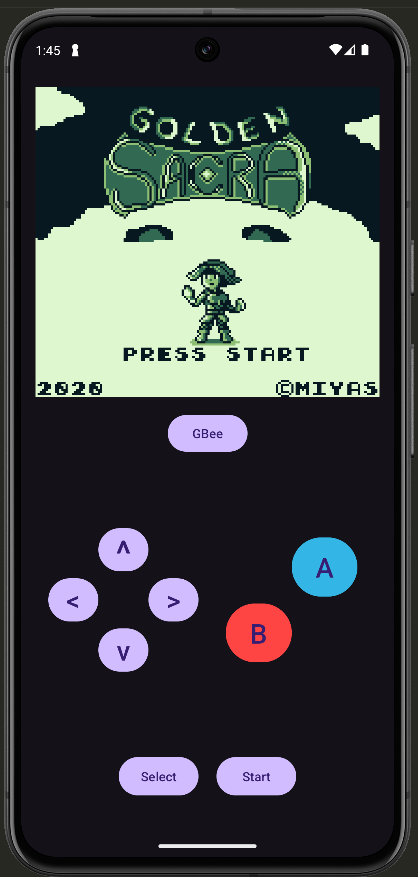
\includegraphics[width=\textwidth]{include/images/design_1_1.png}
        \caption{Diseño inicial en modo Portrait}
        \label{figure:design_1_portrait}
    \end{minipage}
    \hspace{0.05\textwidth}
    \begin{minipage}{0.50\textwidth}
        \centering
        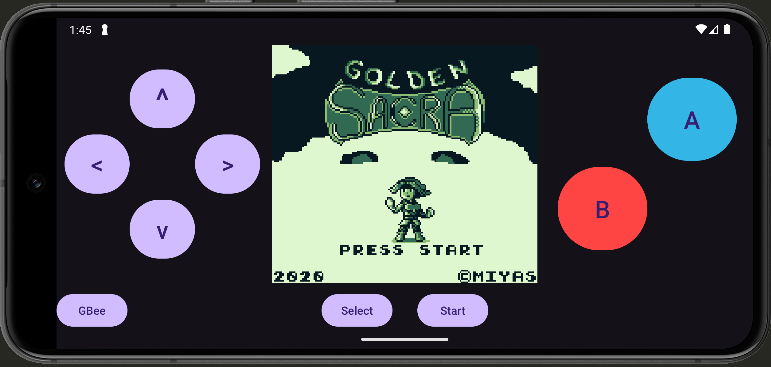
\includegraphics[width=\textwidth]{include/images/design_1_2.png}
        \caption{Diseño inicial en modo Landscape}
        \label{figure:design_1_landscape}
    \end{minipage}
\end{figure}

En la actividad se implementará una función llamada \texttt{configureButtons()}, cuya finalidad será, por un lado, enlazar cada botón del \textit{layout} con una constante que identifique qué botón representa y, por otro, delegar en la función \texttt{setButton(button: View, name: String)} la inicialización de los correspondientes \textit{listeners}.

\begin{lstlisting}[language=Kotlin, caption={Enlace y Lógica de los Botones en la Actividad}, label={code:activityjoypad}]
    private fun configureButtons(){
        setButton(binding.dpadUp, UP_DPAD)
        setButton(binding.dpadDown, DOWN_DPAD)
        setButton(binding.dpadLeft, LEFT_DPAD)
        setButton(binding.dpadRight, RIGHT_DPAD)
        setButton(binding.buttonA, A_BUTTON)
        setButton(binding.buttonB, B_BUTTON)
        setButton(binding.buttonSelect, SELECT_BUTTON)
        setButton(binding.buttonStart, START_BUTTON)
        dbgButton = binding.switchButton
    }

    @SuppressLint("ClickableViewAccessibility")
    private fun setButton(button: View, name: String){
        button.setOnTouchListener { v, event ->
            when (event.action) {
                MotionEvent.ACTION_DOWN -> {
                    //println("Button pressed: $name")
                    IO.setButtonPressed(name, true)
                    true
                }
                MotionEvent.ACTION_UP -> {
                    //println("Button released: $name")
                    IO.setButtonPressed(name, false)
                    v.performClick()
                    true
                }
                else -> false
            }
        }
    }
    
\end{lstlisting}

Ahora, utilizando nuevamente el juego \textit{Golden Sacra}, al pulsar el botón de Start, el emulador debe dar paso del menú principal a la pantalla de juego:

\begin{figure}[H]
    \centering
    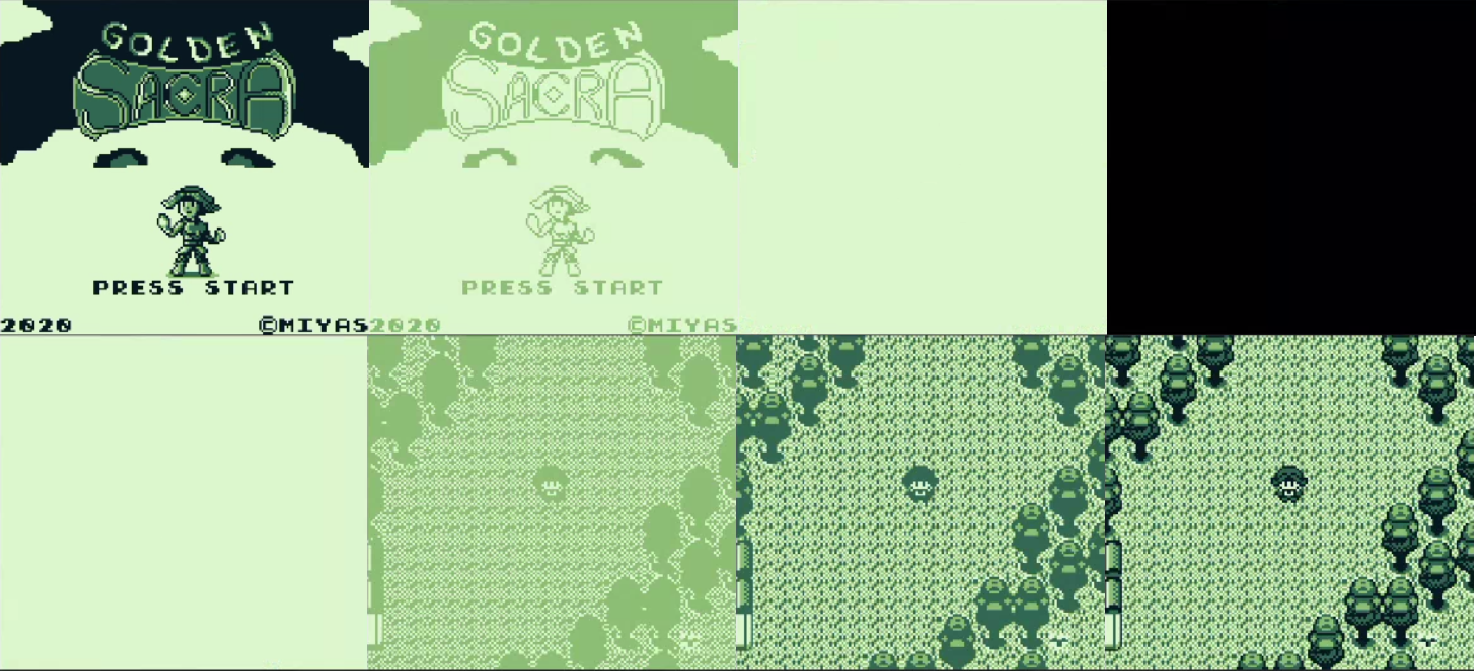
\includegraphics[width=1\textwidth]{include/images/transition_title.png}
    \caption{Paso desde la Pantalla de Título a Juego.}\label{figure:transition_title}
\end{figure}

\section{MainActivity}

A partir de este apartado se enfocará la memoria en lo que es la parte púramente de Android a nivel de aplicación. Se dará comienzo por lo primero que se ve al iniciar la aplicación: el \textit{MainActivity}.
\\\\
Haciendo uso del \hyperref[figure:mockupmenu]{diseño original}, se procede a generar las siguientes clases, estructuras o modificaciones:

\begin{enumerate}
    \item Añadir un Toolbar al layout que tenga dos botones, uno para añadir una ROM y otro para entrar a la configuración.
    \item Añadir un RecyclerView al layout, el cual quedará configurado en el \texttt{onCreate()}.
    \item Generar un Adapter para el RecyclerView, que contendrá la lógica de cómo se van a mostrar las ROMs en pantalla.
    \item Crear un layout para cada elemento del RecyclerView, que contendrá una imágen y el nombre de la ROM.
    \item Aádir dos \textit{listeners}, el primero (clics corto) que indicará que un usuario quiere iniciar una ROM, y otro (clics largos) que indicará que el usuario quiere hacer algo (eliminar o modificar) esa ROM.
    \item Añadir un \textit{listener} al botón de añadir ROM, que abrirá un explorador de archivos para que el usuario seleccione la ROM que quiere añadir.
    \item Copiar y guardar las ROMs añadidas por el usuario en la memoria interna de la aplicación, para que se mantengan entre sesiones, independientemente de si el usuario la ha borrado de la carpeta original a posteriori.
    \item Generar un modelo de SQLite para guardar la información de las ROMs en la base de datos. De esta forma el usuario podrá modificar el título y la imagen utilizada como carátula. 
    \item Añadir un \textit{listener} al botón de configuración, que abrirá una nueva actividad donde se podrá modificar la configuración del emulador.
\end{enumerate}

En la configuración del \texttt{RecyclerView} se debe establecer el \texttt{LayoutManager}, que es el encargado de gestionar la disposición de los elementos en pantalla. En este caso, se utilizará un \texttt{GridLayoutManager} para mostrar las ROMs en una cuadrícula. También se debe establecer el \texttt{Adapter}, que es el encargado de proporcionar los datos al \texttt{RecyclerView}. Para este último punto, se creará una clase \texttt{RomAdapter} que extenderá de \texttt{RecyclerView.Adapter}.
\\\\
A continuación se muestra el código de la actividad principal, donde se inicializa el \texttt{RecyclerView} y se configuran los \textit{listeners}:

\begin{lstlisting}[language=Kotlin, caption={MainActivity - Configuración del RecyclerView.}, label={code:activitymain}]
    private fun createRecyclerView(){

        RomManagement.loadROMSFromDBIfNeeded(this)

        val spanCount = if (resources.configuration.orientation == Configuration.ORIENTATION_LANDSCAPE) {
            3
        } else {
            2
        }

        binding.romGrid.layoutManager = GridLayoutManager(this, spanCount)
        binding.romGrid.itemAnimator = DefaultItemAnimator()

        romAdapter = ROMAdapter(ROMDataSource.roms, spanCount)

        // Click Listener
        romAdapter.setOnItemClickListener { romPosition ->

            val selectedROMTitle = romAdapter.romList[romPosition].title

            if (selectedROMTitle != null) {
                val romEntity =
                    SQLManager.getDatabase(this).romDAO().getROMByTitle(selectedROMTitle)

                if (romEntity != null)
                    startActivity(
                        Intent(this, EmuActivity::class.java)
                            .putExtra(ROM_PATH_EXTRA, romEntity.filePath)
                    )
            }
        }

        romAdapter.setOnLongItemClickListener { romPosition, v ->
            showPopupMenu(v, romPosition)
            true
        }

        binding.romGrid.adapter = romAdapter
    }
\end{lstlisting}

Gracias al \texttt{GridLayoutManager}, podemos determinar cuántas ROMs mostrar por fila. Se han definido 2 para el modo \textit{portrait} y 3 para el \textit{landscape}. También se asigna un animador de ítems por defecto para gestionar animaciones al añadir, eliminar o mover elementos.
\\\\
Posteriormente, se instancia el adaptador \texttt{ROMAdapter} pasando la lista de ROMs y el número de columnas. Como se ha expuesto antes, se configuran los \textit{listeners} para los dos tipos de clic. Cuando se selecciona una ROM, se obtiene su título y, si está disponible, se consulta a la base de datos para recuperar la entidad correspondiente. Si se encuentra la ROM, se lanza el intent para pasar al \texttt{EmuActivity} y se le pasa la ruta del archivo como extra.
\\\\
A continuación, se configura el \textit{listener} para el clic largo. En este caso, se muestra un menú emergente relacionado con la ROM seleccionada. 
\\\\
Finalmente, se asigna el adaptador al \texttt{RecyclerView}, completando así la configuración.
\\\\
Por otro lado, se deben implementar los \textit{listeners} de los botones que permiten añadir ROMs y entrar a la pantalla de ajustes. Al mismo tiempo que configuramos el \texttt{RecyclerView}, enlazaremos los dos botones definidos en el layout con dos \textit{launchers}.
\\\\
El launcher del botón de añadir, comprobará primero si el fichero ya existe en la memoria interna mediante la función \texttt{RomManagement.fileAlreadyExists(context: Context, uri: Uri)}. En caso negativo, copiará y añadirá el fichero a la memoria privada de la aplicación y, si esta operación tiene éxito, la añadirá también al \textit{data source} y a la base de datos. Por último, notificará al \textit{adapter} de que un nuevo objeto se ha insertado para que la vista se actualice correctamente.
\\\\
El launcher del botón de ajustes simplemente generará un \textit{intent} que delegará el trabajo en otra actividad, la cual se implementará posteriormente.

\subsection{SQL ROM Data}

Para guardar, obtener y listar todas las ROMs y sus datos, se van a generar los siguientes archivos:
\begin{itemize}
    \item \textbf{ROM}: \textit{Data Class} que va a contener un entero como identificador, una cadena de texto para el título y una segunda cadena de texto para la imagen.
    \item \textbf{ROMDataSource}: Contiene el listado de todas las ROMs en tiempo de ejecución.
    \item \textbf{ROMManagement}: El manejador de las ROMs, contiene toda la lógica para guardar, eliminar y obtener las ROMs de la memoria privada. Se implementará como un \textbf{singleton}.
    \item \textbf{ROMDao}: Un \textit{Data Access Object} que define la interfaz SQL. Contendrá funciones para insertar, actualizar, obtener y eliminar ROMs.
    \item \textbf{ROMEntity}: Un \textit{Data Class} parecido al de ROM, pero con propiedades para la ruta donde se almacena el fichero original, la ruta donde se almacene el archivo de guardado, la fecha en la que la ROM fue añadida, y el tipo (DMG o CGB).
\end{itemize}

\subsubsection{ROM Management}
A continuación se explica el \texttt{ROMManagement} más en profundidad:
\\\\
La función principal es \texttt{addROM()}, que permite registrar una nueva ROM. Este método limpia el nombre del archivo recibido, eliminando extensiones y caracteres indeseados para generar un título más legible. A continuación, se crea una entidad \texttt{ROMEntity} que representa la ROM con su ruta, título, tipo y fecha de añadido. Esta entidad se guarda en la base de datos y se añade a la lista de ROMs en memoria mediante \texttt{saveROMToDatabaseAndDataSource()}.

\begin{lstlisting}[language=Kotlin, caption={ROM Management - Añadir una ROM.}, label={code:romManagementAddRom}]
    fun addROM(context: Context, romPath: String, romTitle: String) {

        val title = romTitle.replace(Regex("\\.gbc?"), "").replace(Regex("_"), " ")
        val type = if(romTitle.contains(".gbc")) "gbc" else "gb"

        val newROM = ROMEntity(
            filePath = romPath,
            title = title,
            imageRes = null,
            saveFilePath = null,
            addedDate = System.currentTimeMillis(),
            type = type
        )

        saveROMToDatabaseAndDataSource(newROM, context)
    }

    private fun saveROMToDatabaseAndDataSource(rom: ROMEntity, context: Context) {
        val db = SQLManager.getDatabase(context)
        val id = db.romDAO().insertROM(rom)

        ROMDataSource.addROM(ROM(title = rom.title, id = id.toInt()))
    }
\end{lstlisting}

En cuanto a la eliminación de ROMs, la función \texttt{deleteRom()} permite borrarlas tanto de la base de datos como del almacenamiento y las preferencias asociadas. Si se elimina correctamente, también se actualiza la fuente de datos en memoria y se informa al usuario con un mensaje emergente. Internamente, este proceso utiliza \texttt{deleteROMFile()}, que se encarga de borrar físicamente los archivos relacionados y actualizar la base de datos.
\\\\
Existe una clase llamada \texttt{FileManager}, que podría definirse como una capa inferior en cuanto al mantenimiento de archivos. Contiene una implementación bastante común, por lo que se va a omitir la explicación su código.

\begin{lstlisting}[language=Kotlin, caption={ROM Management - Eliminar una ROM.}, label={code:romManagementDeleteRom}]
    fun deleteRom(context: Context, rom: ROM, position: Int): Boolean{
        val dao = SQLManager.getDatabase(context).romDAO()
        val romEntity = dao.getROMByTitle(rom.title ?: "")
        if(romEntity != null) {
            // Delete private file and database entry
            if(deleteROMFile(context, romEntity)) {

                // Delete from Shared Preferences
                val preferences = context.getSharedPreferences(romEntity.id.toString(), Context.MODE_PRIVATE)
                val editor = preferences.edit()
                editor.clear()
                editor.apply()

                // Delete from Data Source
                ROMDataSource.roms.removeAt(position)

                Toast.makeText(context, "${rom.title} has been deleted", Toast.LENGTH_SHORT).show()
                return true
            }
        }
        Toast.makeText(context, "An error has occurred", Toast.LENGTH_SHORT).show()
        return false
    }

    private fun deleteROMFile(context: Context, rom: ROMEntity?) : Boolean {
        val romDao = SQLManager.getDatabase(context).romDAO()

        // Delete file from private storage
        if(rom != null) {
            val filepath = rom.filePath
            val imagePath = rom.imageRes

            if (filepath.isNotEmpty()) {
                val file = File(filepath)
                if (file.exists()) {
                    file.delete()
                }
            }
            // Delete from DB
            romDao.deleteROM(rom)

            // Delete game cover if needed
            if(imagePath != null)
                FileManager.deleteFileFromPrivateStorage(imagePath)

            return true
        }

        return false
    }
\end{lstlisting}

Por último, la función \texttt{loadROMSFromDBIfNeeded()} sincroniza la fuente de datos en memoria con el contenido de la base de datos. Si el número de ROMs en memoria no coincide con el de la base de datos, las recarga todas, teniendo en cuenta también posibles valores almacenados en \texttt{SharedPreferences}, como portadas personalizadas o nombres editados.

\begin{lstlisting}[language=Kotlin, caption={ROM Management - Recarga de ROMs en Memoria.}, label={code:romManagementReloadRoms}]
    fun loadROMSFromDBIfNeeded(context: Context){
        val romDao = SQLManager.getDatabase(context).romDAO()
        val allRoms = romDao.getAllROMs()
        if(ROMDataSource.roms.size != allRoms.size){
            ROMDataSource.roms.clear()
            allRoms.forEach {
                val preferences = context.getSharedPreferences(it.id.toString(), Context.MODE_PRIVATE)
                val prefTitle = preferences.getString(TITLE_KEY, it.title)
                val prefImage = preferences.getString(COVER_KEY, it.imageRes)
                ROMDataSource.addROM(ROM(id = it.id, title = prefTitle, imageRes = prefImage))
            }
        }
    }
\end{lstlisting}

\subsection{ROM Adapter}
Como se ha explicado ya, el \texttt{ROMAdapter} es el encargado de gestionar la forma en que se muestran las ROMs en el \texttt{RecyclerView}. Este adaptador extiende de \texttt{RecyclerView.Adapter} y se inicializa con una lista de ROMs y el número de columnas que se van a mostrar.
\\\\
Contiene una clase interna llamada \texttt{ViewHolder}, que se encarga de gestionar la vista de cada elemento. Esta clase contiene una referencia a la vista de la ROM y a su imagen, así como los métodos para enlazar los datos de la ROM con la vista.
\\\\
A cada ROM, por defecto, se le asigna una imagen predeterminada que se encuentra en la carpeta de recursos. Esta imagen se puede cambiar posteriormente a través de un \textit{dialog} que permite al usuario seleccionar una imagen de su galería.
\\\\
A cada view se le hace el inflado mediante un layout que define cómo representar cada objeto de forma individual. Este layout se encuentra en la carpeta de recursos y contiene un \texttt{ImageView} y un \texttt{TextView} para mostrar la imagen y el título de la ROM, respectivamente. El layout se infla en el método \texttt{onCreateViewHolder()} del adaptador.

\begin{lstlisting}[language=Kotlin, caption={ROM Adapter.}, label={code:romAdapter}]
    class ROMAdapter(val romList: MutableList<ROM>, private val spanCount: Int)  :
        RecyclerView.Adapter<ROMAdapter.ViewHolder?>() {

        [...]

        override fun onCreateViewHolder(parent: ViewGroup, viewType: Int): ViewHolder {
            val v: View = LayoutInflater.from(parent.context).inflate(R.layout.rom_grid_item, parent, false)

            [...]

        class ViewHolder(v: View) : RecyclerView.ViewHolder(v) {
            private var name: TextView
            private var icon: ImageView
            private val view = v

            fun bind(it: ROM) {
                name.text = it.title

                icon.setImageResource(R.drawable.rom_icon)

                if(it.imageRes != null) {
                    val file = File(it.imageRes!!)
                    if (file.exists())
                        icon.setImageURI(Uri.fromFile(file))
                }
            }

            init {
                name = view.findViewById(R.id.rom_title)
                icon = view.findViewById(R.id.rom_image)
            }
        }
\end{lstlisting}

Una vez implementados los puntos anteriores, la aplicación debe permitir añadir y visualizar las ROMs en la página principal:

\begin{figure}[H]
    \centering
    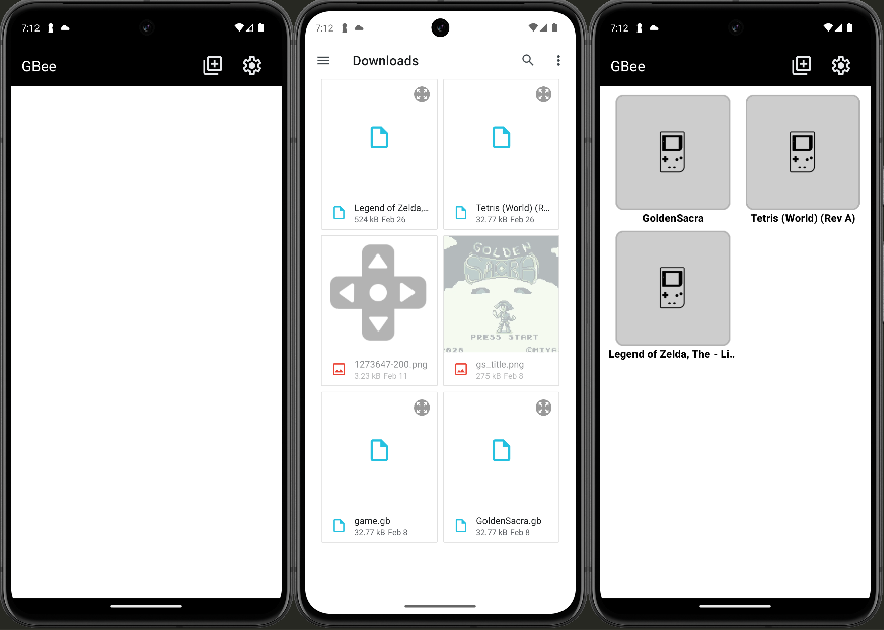
\includegraphics[width=0.9\textwidth]{include/images/add_rom.png}
    \caption{MainActivity - Añadir ROMs al Emulador.}\label{figure:addRom}
\end{figure}

\section{SettingsActivity}
La actividad de configuración es la encargada de gestionar la configuración del emulador. Esta actividad se lanza desde el \texttt{MainActivity} y permite al usuario modificar distintas opciones del emulador, como la paleta de colores o modificar la interfaz de juego. Implementa la interfaz \texttt{OnPreferenceStartFragmentCallback}, lo que permite mostrar fragmentos secundarios de configuración según las interacciones del usuario.
\\\\
En el método \texttt{onCreate()} se incluye una barra de herramientas y un contenedor de fragmentos. La barra se configura para permitir la navegación hacia atrás. Por otro lado, se obtiene el valor del identificador de juego a través del \textit{intent} que ha lanzado la actividad anterior. Este identificador determina si se deben mostrar las preferencias asociadas a un juego específico (\texttt{GameSettingsFragment}) o las preferencias generales de la aplicación (\texttt{SettingsFragment}). Si el identificador es distinto de -1, se interpreta que la configuración está vinculada a un juego concreto.

\begin{lstlisting}[language=Kotlin, caption={SettingsActivity - Inicialización.}, label={code:settingsActivityInit}]
    class SettingsActivity : AppCompatActivity(), PreferenceFragmentCompat.OnPreferenceStartFragmentCallback {

    private lateinit var binding: ActivitySettingsBinding
    private var gameId = -1

    override fun onCreate(savedInstanceState: Bundle?) {
        super.onCreate(savedInstanceState)

        binding = ActivitySettingsBinding.inflate(layoutInflater)
        setContentView(binding.root)
        setSupportActionBar(binding.toolbar)

        supportActionBar?.apply {
            setDisplayHomeAsUpEnabled(true)
        }

        gameId = intent.getIntExtra(GAME_ID, -1)

        if (gameId != -1) {
            supportFragmentManager
                .beginTransaction()
                .replace(R.id.fragment_container, GameSettingsFragment(gameId))
                .commit()
        } else if (savedInstanceState == null) {
            supportFragmentManager
                .beginTransaction()
                .replace(R.id.fragment_container, SettingsFragment())
                .commit()
        }

        [...]
\end{lstlisting}

La función \texttt{onPreferenceStartFragment()} se ejecuta cuando el usuario selecciona una opción de configuración que abre un nuevo fragmento. En este método se instancia dinámicamente el nuevo fragmento a partir de la clase especificada en la preferencia. Además, se le pasan los extras necesarios, como el identificador visto previamente. El fragmento se añade a la pila de retroceso para que el usuario pueda navegar hacia atrás de forma natural.

\begin{lstlisting}[language=Kotlin, caption={SettingsActivity - Selección de Otro Fragmento.}, label={code:settingsActivitySelect}]
    override fun onPreferenceStartFragment(
        caller: PreferenceFragmentCompat,
        pref: Preference
    ): Boolean {
        val fragment = supportFragmentManager.fragmentFactory.instantiate(
            classLoader,
            pref.fragment!!
        )

        pref.extras.putInt(GAME_ID, intent.getIntExtra(GAME_ID, -1))

        fragment.arguments = pref.extras

        supportFragmentManager.beginTransaction()
            .replace(R.id.fragment_container, fragment)
            .addToBackStack(null)
            .commit()
        return true
    }
\end{lstlisting}

El \texttt{SettingsFragment} que se utiliza por defecto en la actividad, utiliza un archivo XML de preferencias, donde vienen definidos y enlazados con sus respectivas clases todos los subfragmentos a los que se puede navegar. Además, utilizar fragmentos ofrece la posibilidad de añadir toda la lógica que se necesite según qué situación.

\begin{lstlisting}[language=Kotlin, caption={SettingsActivity - Archivo de Preferencias.}, label={code:settingsActivityPreferences}]
    <PreferenceScreen
        xmlns:android="http://schemas.android.com/apk/res/android">

        <Preference
            android:key="video_settings"
            android:title="Video"
            android:icon="@drawable/video_settings_vector"
            android:summary="Adjust video settings"
            android:fragment="es.atm.gbee.core.fragments.VideoSettingsFragment" />

        <Preference
            android:key="audio_settings"
            android:title="Audio"
            android:icon="@drawable/music_note_vector"
            android:summary="Adjust audio settings"
            android:fragment="es.atm.gbee.core.fragments.AudioSettingsFragment" />

        [...]
\end{lstlisting}

Por último, se ha implementado el método \texttt{onSupportNavigateUp()}, el cual se encarga de devolver el control a la actividad anterior cuando el usuario pulsa el botón de retroceso en la barra de herramientas. Se crea un \textit{intent} con el identificador de juego actual para devolverlo como resultado, y se lanza \texttt{onBackPressedDispatcher} para que la navegación hacia atrás se gestione correctamente.
\\\\
El resultado es el que se puede ver en las siguientes figuras:

\begin{figure}[H]
    \centering
    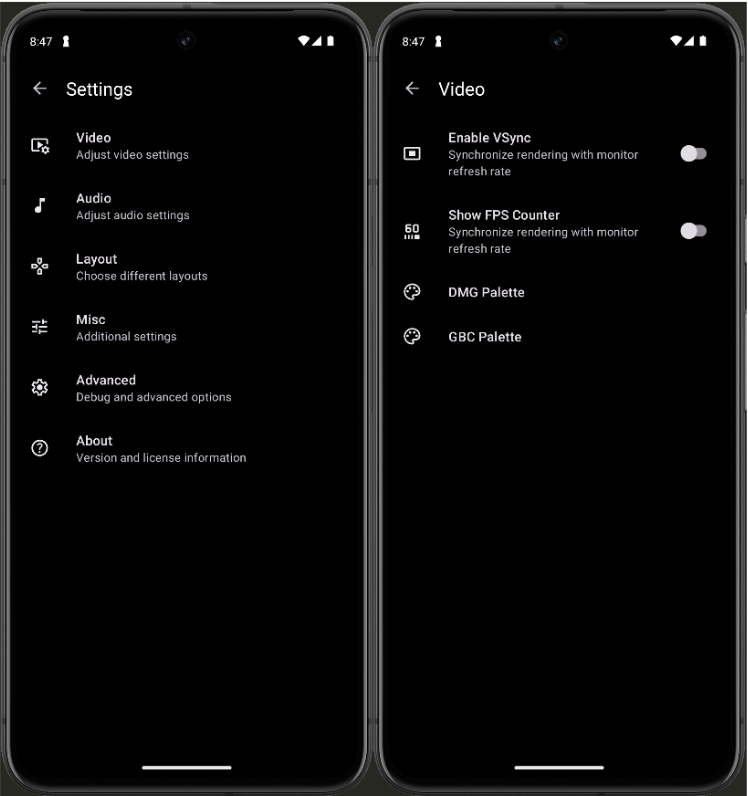
\includegraphics[width=0.75\textwidth]{include/images/settings_fragments.png}
    \caption{Transición entre Fragmentos en la Pantalla de Ajustes.}\label{figure:settingsFragments}
\end{figure}

Los ajustes que el usuario tome, tanto de forma general como de forma individual por cada juego, se guardarán mediante \textit{SharedPreferences}. Existen excepciones como la carátula que el usuario quiera configurar a cada juego, que se deben guardar en memoria privada.
\\\\
A continuación se muestra un ejemplo en el que el usuario modifica la portada de un juego:

\begin{figure}[H]
    \centering
    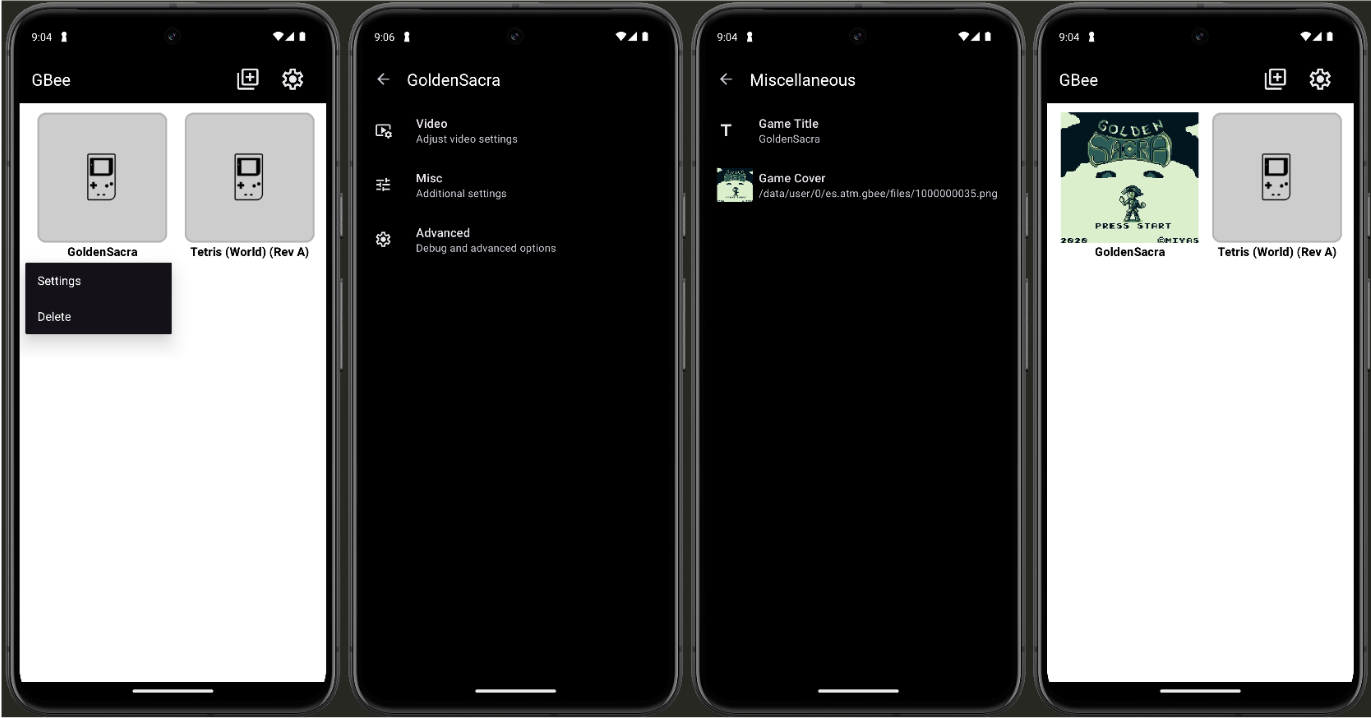
\includegraphics[width=1\textwidth]{include/images/settings_misc.png}
    \caption{Modificación de la Portada de un Juego.}\label{figure:miscFragment}
\end{figure}

\subsection{Skins}

El emulador permite al usuario cambiar la apariencia de la interfaz de juego. Para ello, se ha implementado un sistema de \textit{skins} que permite personalizar la apariencia del emulador. Cada skin se define mediante una entidad SQL que contiene los colores, imágenes y estilos de los distintos elementos de la interfaz.
\\\\
El sistema de \textit{skins} se basa en el uso de \texttt{SharedPreferences} para almacenar la configuración de la skin seleccionada por el usuario. Al iniciar el emulador, se carga la skin seleccionada y se aplican los estilos correspondientes a los distintos elementos de la interfaz.
\\\\
De la misma manera que se ha hecho con la página principal que muestra todas las ROMs, se ha generado las siguientes clases y estructuras:

\begin{itemize}
    \item \textbf{Skin}: \textit{Data Class} que contiene un entero como identificador, una cadena de texto para el título, un color para el fondo, y un array de bytes para cada uno de los botones.
    \item \textbf{SkinDataSource}: Contiene el listado de todas las skins en tiempo de ejecución.
    \item \textbf{SkinManagement}: El manejador de las skins, contiene toda la lógica para guardar, eliminar y obtener las skins de la base de datos. Se implementa también como un \textbf{singleton}.
    \item \textbf{SkinDao}: Un \textit{Data Access Object} que define la interfaz SQL. Contiene funciones para insertar, actualizar, obtener y eliminar skins.
    \item \textbf{SkinEntity}: Un \textit{Data Class} muy similar al modelo de Skin.
    \item \textbf{SkinAdapter}: Un adaptador para el \texttt{RecyclerView} que muestra las skins disponibles. Contiene la lógica de cómo se van a mostrar las skins en pantalla.
    \item \textbf{Skin Item}: Un layout para cada elemento del \texttt{RecyclerView}, que contendrá una imágen y el nombre de la skin.
    \item \textbf{CustomSkinsActivity}: Una actividad que permite al usuario seleccionar una skin personalizada. Contiene un \texttt{RecyclerView} que muestra todas las skins disponibles y permite al usuario seleccionar una de ellas.
    \item \textbf{CreateCustomSkinActivity}: Una actividad que permite al usuario crear una skin personalizada. Muestra un layout por defecto en el que el usuario puede seleccionar los colores y las imágenes de los distintos elementos de la interfaz.
\end{itemize}

La diferencia con el \texttt{ROMAdapter} es que no se va a utilizar un \texttt{GridLayoutManager}, ya que se van a listar en forma de lista. Además, siempre aparecerá una skin por defecto, que vendrá preconfigurada con la aplicación y que los usuarios pueden utilizar pero no eliminar ni editar.
\\\\
La lógica del manejador de skins es muy similar a la de las ROMs, con la diferencia de que no se están manejando ficheros, solamente entidades SQL. Por otro lado, la configuración del \textit{RecyclerView} y los \textit{listeners} también sigue el mismo patrón. Por ello, vamos a obviar la parte de código para evitar redundancias.
\\\\
El emulador comenzará utilizando la skin predeterminada, pero el usuario podrá cambiarla en cualquier momento tanto por otra skin que genere como por el diseño original que utiliza botones comunes de Android.

\subsection{Diseño de Skin Predeterminada}
Para la skin predeterminada se ha optado por un diseño sencillo, que no sature al usuario y que permita una buena visibilidad de los elementos. Se ha utilizado un fondo amarillo con un color negro para los botones. Dar las gracias a Carla Maciá Díez por la ayuda proporcionada con todos los elementos. A continuación se muestra el diseño de todos los elementos de la skin predeterminada:

\begin{figure}[H]
    \centering
    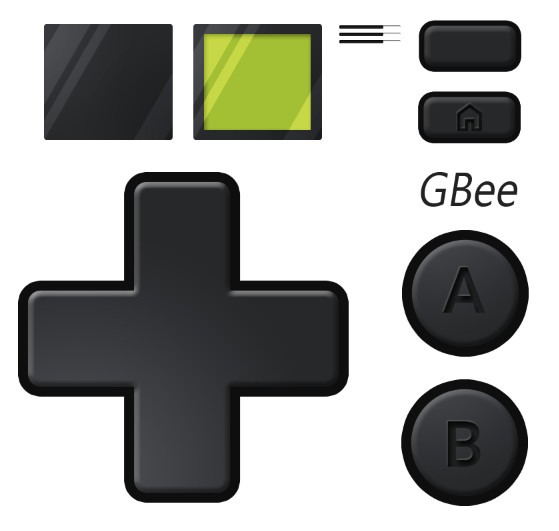
\includegraphics[width=0.8\textwidth]{include/images/new_design_elements.png}
    \caption{Nuevos Diseños para los Elementos de la Interfaz de Juego.}\label{figure:newDesignElements}
\end{figure}

\cleardoublepage